
% Template for Elsevier CRC journal article
% version 1.1 dated 16 March 2010

% This file (c) 2010 Elsevier Ltd.  Modifications may be freely made,
% provided the edited file is saved under a different name

% This file contains modifications for Procedia Computer Science
% but may easily be adapted to other journals

% Changes since version 1.0
% - elsarticle class option changed from 1p to 3p (to better reflect CRC layout)

%-----------------------------------------------------------------------------------

%% This template uses the elsarticle.cls document class and the extension package ecrc.sty
%% For full documentation on usage of elsarticle.cls, consult the documentation "elsdoc.pdf"
%% Further resources available at http://www.elsevier.com/latex

%-----------------------------------------------------------------------------------

%%%%%%%%%%%%%%%%%%%%%%%%%%%%%%%%%%%%%%%%%%%%%%
%%%%%%%%%%%%%%%%%%%%%%%%%%%%%%%%%%%%%%%%%%%%%%
%%                                          %%
%% Important note on usage                  %%
%% -----------------------                  %%
%% This file must be compiled with PDFLaTeX %%
%% Using standard LaTeX will not work!      %%
%%                                          %%
%%%%%%%%%%%%%%%%%%%%%%%%%%%%%%%%%%%%%%%%%%%%%%
%%%%%%%%%%%%%%%%%%%%%%%%%%%%%%%%%%%%%%%%%%%%%%

%% The '3p' and 'times' class options of elsarticle are used for Elsevier CRC
\documentclass[3p,times]{elsarticle}

%% The `ecrc' package must be called to make the CRC functionality available
\usepackage{ecrc}
\usepackage{setspace}
\usepackage{algcompatible}
\usepackage[usenames,dvipsnames]{color}
\usepackage{amsthm,amsmath}
\newtheorem{definition}{Definition}
\usepackage{graphicx}% Include figure files
\usepackage{dcolumn}% Align table columns on decimal point
\usepackage{bm}% bold math
\usepackage{hyperref}% add hypertext capabilities
\usepackage[mathlines]{lineno}
\usepackage{bbm,booktabs}
\usepackage{csquotes}
\bibliographystyle{elsarticle-num}


%% The ecrc package defines commands needed for running heads and logos.
%% For running heads, you can set the journal name, the volume, the starting page and the authors

%% set the volume if you know. Otherwise `00'
\volume{00}

%% set the starting page if not 1
\firstpage{1}

%% Give the name of the journal
\journalname{Social Networks}

%% Give the author list to appear in the running head
%% Example \runauth{C.V. Radhakrishnan et al.}
\runauth{}

%% The choice of journal logo is determined by the \jid and \jnltitlelogo commands.
%% A user-supplied logo with the name <\jid>logo.pdf will be inserted if present.
%% e.g. if \jid{yspmi} the system will look for a file yspmilogo.pdf
%% Otherwise the content of \jnltitlelogo will be set between horizontal lines as a default logo

%% Give the abbreviation of the Journal.
\jid{SN}

%% Give a short journal name for the dummy logo (if needed)
\jnltitlelogo{Social Networks}

%% Hereafter the template follows `elsarticle'.
%% For more details see the existing template files elsarticle-template-harv.tex and elsarticle-template-num.tex.

%% Elsevier CRC generally uses a numbered reference style
%% For this, the conventions of elsarticle-template-num.tex should be followed (included below)
%% If using BibTeX, use the style file elsarticle-num.bst

%% End of ecrc-specific commands
%%%%%%%%%%%%%%%%%%%%%%%%%%%%%%%%%%%%%%%%%%%%%%%%%%%%%%%%%%%%%%%%%%%%%%%%%%

%% The amssymb package provides various useful mathematical symbols
\usepackage{amssymb}
%% The amsthm package provides extended theorem environments
%% \usepackage{amsthm}

%% The lineno packages adds line numbers. Start line numbering with
%% \begin{linenumbers}, end it with \end{linenumbers}. Or switch it on
%% for the whole article with \linenumbers after \end{frontmatter}.
%% \usepackage{lineno}

%% natbib.sty is loaded by default. However, natbib options can be
%% provided with \biboptions{...} command. Following options are
%% valid:

%%   round  -  round parentheses are used (default)
%%   square -  square brackets are used   [option]
%%   curly  -  curly braces are used      {option}
%%   angle  -  angle brackets are used    <option>
%%   semicolon  -  multiple citations separated by semi-colon
%%   colon  - same as semicolon, an earlier confusion
%%   comma  -  separated by comma
%%   numbers-  selects numerical citations
%%   super  -  numerical citations as superscripts
%%   sort   -  sorts multiple citations according to order in ref. list
%%   sort&compress   -  like sort, but also compresses numerical citations
%%   compress - compresses without sorting
%%
%% \biboptions{comma,round}

% \biboptions{}

% if you have landscape tables
\usepackage[figuresright]{rotating}

% put your own definitions here:
%   \newcommand{\cZ}{\cal{Z}}
%   \newtheorem{def}{Definition}[section]
%   ...

% add words to TeX's hyphenation exception list
%\hyphenation{author another created financial paper re-commend-ed Post-Script}

% declarations for front matter

\begin{document}

\begin{frontmatter}

%% Title, authors and addresses

%% use the tnoteref command within \title for footnotes;
%% use the tnotetext command for the associated footnote;
%% use the fnref command within \author or \address for footnotes;
%% use the fntext command for the associated footnote;
%% use the corref command within \author for corresponding author footnotes;
%% use the cortext command for the associated footnote;
%% use the ead command for the email address,
%% and the form \ead[url] for the home page:
%%
%% \title{Title\tnoteref{label1}}
%% \tnotetext[label1]{}
%% \author{Name\corref{cor1}\fnref{label2}}
%% \ead{email address}
%% \ead[url]{home page}
%% \fntext[label2]{}
%% \cortext[cor1]{}
%% \address{Address\fnref{label3}}
%% \fntext[label3]{}

%\dochead{}
%% Use \dochead if there is an article header, e.g. \dochead{Short communication}

\title{Hierarchical Structure in Social Networks}

%% use optional labels to link authors explicitly to addresses:
%% \author[label1,label2]{<author name>}
%% \address[label1]{<address>}
%% \address[label2]{<address>}

\author[au1]{Cynthia Cook\footnote{Authors are listed in alphabetical order but all contributed equally to this publication.}} 
\author[au2]{Matthew J. Denny}
\author[au3]{Mitchell Goist} 
\author[au4]{Timmy Huynh}

\address[au1]{Department of Statistics cmc496@psu.edu}
\address[au2]{Department of Political Science, mdenny@psu.edu}
\address[au3]{Department of Political Science mlg307@psu.edu}
\address[au4]{Department of Sociology and Criminology, tnh133@psu.edu}

\begin{abstract}

\end{abstract}

\begin{keyword}
Hierarchy \sep Network \sep Power

%% MSC codes here, in the form: \MSC code \sep code
%% or \MSC[2008] code \sep code (2000 is the default)

\end{keyword}

\end{frontmatter}

%%
%% Start line numbering here if you want
%%
% \linenumbers


\section{Introduction}
\label{sec:introduction}

Hierarchy is an important feature of many organizations, such as firms, social clubs, and military units. Formally, we can define a hierarchy as a system where people or groups are ranked according to status or authority. Yet it is difficult to operationalize this definition for measurement and comparison. There has been a great deal of research on power and status in groups and organizations, but most of this research relies on measurements defined over domain specific rankings, such as job titles. At the same time, networks scholars have defined a number of broadly applicable hierarchy metrics based on network structure, but these metrics are not necessarily grounded in meaningful sociological concepts of status and authority. While some social theorists have noted that a network-oriented perspective of the ``sociospatial and organizational model [of a network]" can explicate the ``sources of social power," \cite{mann1986sources} they have generally not delved into the methodologies through which to fully explore such power dynamics. In this paper, we seek to bring together these two areas of research, and to develop a framework for measuring hierarchy in social networks that is both generally applicable and exhibits a high degree of construct validity.

In this study: we describe theories of hierarchy in social science, formally state and explain commonly used measures for network hierarchy, and illustrate the ways in which these measures correspond and diverge when applied to a wide variety of observed social networks. We find that the twelve measures of hierarchy we consider can be mapped onto several dimensions of hierarchy derived from the sociological literature. We also find wide variation in the theoretical and empirical suitability of the measures we consider to the measurement of hierarchy across different types of social networks (e.g. communication, friendship, exchange, etc.). We conclude that there is not one-size fits all measure of hierarchy, and that carefule theoretical guidance is necessary in selecting an appropriate measure or set of measures for a particular domain.

%; demonstrate how these measures respond to network features;

% \subsection{Problem Statement}
% \begin{flushleft}
% 	How do we define and measure hierarchy in (directed) social networks? We need to relate sociological conceptions of hierarchy and power to network measures. In developing this framework we intend to compare analytical and statistical approaches to measurement on both synthetic and real world datasets. In particular there are several key questions we must address.
% \end{flushleft}
% \begin{enumerate}
% 	\item Is an analytical or statistical measure of network hierarchy more appropriate for our  goals?
% 	\item Can we capture all or even most salient dimensions of hierarchy as defined in the sociological literature in a single measure?
% 	\item Can our measure be extended to undirected networks?
% \end{enumerate}

 

\section{Theorizing Hierarchy in Networks}
Much research has noted the importance of network structure for a variety of outcomes.\footnote{For a review of many of these network structures, see \cite{smith2005networks}.} However, little has been conceptualized regarding a generalizable, meaningful, and substantive interpretation into the differential set of relations within a network that lead to localized differences within the broader network structure. %Is there another way to phrase this sentence? --Mitch%
In other words, from the overall network structure may emerge particular network-specific traits of the nodes that may give higher ``prominence" to certain nodes over other nodes. Part of the reason for this gap in the literature is that network scientists and researchers have used a myriad of terms and phrases to describe network concepts that largely approximate one another, so a consensus had been difficult if not impossible to achieve.

Network analysis has become increasingly important in understanding social relations, especially in recent years as advances in computational capacity have allowed for a variety of analytical tools and methods that the theory had long suggested could be possible. In this regard, then, scholars have been puzzling for at least half a century about how mapping social networks leads to a greater understanding of human interactions. Indeed, decades ago, sociologist Harrison White had noted that although a network ``structure is essentially local, a matter of pair relations," ``[n]o satisfactory theory of these complex interrelations [of pairs] has yet been proposed" \cite[p. 172-173]{white2007catnets}. More recently, the quantification of social networks has essentially allowed for a ``geometry of sociology," which ``in the context of network analysis show[s] how fruitful the geometric modeling of systems is, or [...] how important a geometry of spaces of social interactions is" \cite[p. 218]{kluver2000dynamics}. Indeed, ``[t]he geometrical rules represent those characteristics of a system which are usually called the 'structure' of the system and which have been analyzed rather thoroughly in social network analysis" \cite[p. 102]{kluver2000dynamics}. As certain more socially-oriented perspectives on the mechanisms of society come more into vogue, the importance of understanding, conceptualizing, and analyzing social relations in the context of other types of interactions grows ever more relevant. As popularized in sociology around the 1980s, this notion can be referred to as ``embeddedness": ``the argument that the behavior and institutions to be analyzed are so constrained by ongoing social relations that to construe them as independent is a grievous misunderstanding" \cite[p. 162]{granovetter2007economic}. Instead of focusing on various political, social, or economic processes as isolated, the ``embeddedness argument stresses instead the role of concrete personal relations and structures (or 'networks') of such relations in generating trust and discouraging malfeasance" \cite[p. 167]{granovetter2007economic}, with the extent of a network's importance to these other processes as ``depend[ing] very much on how the network of social relations is structured" \cite[p. 168-169]{granovetter2007economic}. For example, in an earlier work, Granovetter conjectured on the ``strength of weak ties," wherein weaker connections in a network proved to have more influence across the network than stronger ones because they were better able to connect otherwise-disparate communities \cite{granovetter1973strength}. Similarly, Bonacich \cite{bonacich1987power} had noted that centrality in a network did not always correlate to power and influence. Instead, drawing on exchange theory, power was drawn more from how dependent actors in a network were on other actors. Indeed, factoring in characteristics of the actors and nodes in a network really helps to flesh out more substantive interpretations. By layering on how actors relate to one another across multiple types of networks, Mizruchi \cite{mizruchi1996interlocks} analyzed how corporate executives wield more influence by being ``interlocked" in more overlapping networks, such as being on multiple boards of directors or exclusive social clubs.

These various studies in the social sciences have all approached power and influence in networks in different ways, but as such, they have also all hinted at the emergent hierarchical structure within the studied networks by explicitly or tacitly suggesting differences in power between nodes. To be clear though, the power and hierarchy of actors in the network exist \textit{because of the network}. Outside of a network structure, the different categories of power lose meaning without the relations as defined by the network. White alluded to this relationality as follows:
\begin{displayquote}
Placement in a cat[egory] in this system is meaningful only within the context of the whole structure formed by the categories. A hierarchical system of social classes is an example. One is not upper class because of some intrinsic attribute but in contrast to being lower class. [...] In this simple case of two social classes one could just say membership is a relative matter, but the word context better conveys the complexity of assignment in more complex systems of categories which form structures. \cite[p. 177]{white2007catnets}
\end{displayquote}
<<<<<<< Local Changes
When we understand societal processes and institutions under a theoretical framework oriented around social relations, we're actually invoking much of the main ideas of sociologist Michael Mann, who comprehends society as ``a network of social interaction" \cite{mann1986sources}. Mann's work in essence calls for a better discernment of the complexity of human social relations and needs, as opposed to Mann’s critique of past theories focusing too much as ``simple totalities" instead. Indeed, he says: ``Societies are constituted of multiple overlapping and intersecting sociospatial networks of power" \cite[p. 1]{mann1986sources}. In light of Mann's broader work, contemporary scholars note that ``[i]n terms of scope and ambition, this project [of Mann's] rivals the social thought of Marx and Weber" \cite[p. 338]{schroeder2007mann}, and his theorizing on the ``relations \textit{between} states" has filled a void that in general, ``[s]ociology has thus been unable to deal with [...] [regarding] contemporary social change" \cite[p. 339-340; emphasis in original]{schroeder2007mann}. This ``project" conceives of the power differentials in society as explained through his IEMP model (or ``the four organizational means and my IEMP [ideological, economic, military, and political] model of organized power" \cite[p. 2-3]{mann1986sources}). Thus, although Mann doesn't explicitly note there is a network ``hierarchy" per se (just as most social theorists and network scientists frame ``hierarchy in networks" differently), he does discuss how the organization of different network structures lead to differences in power, which for our purposes implies a ``power" hierarchy. While the ``distinctive thrust of all of Mann's work is that it is impossible to examine power [...] without analysing the interrelationships between the four separate networks" \cite[p. 339]{schroeder2007mann}, Mann's typologies of power, though, are more generalizable and thus are arguably more relevant in understanding hierarchy irrespective of Mann's IEMP model. In brief, Mann argues that ``power can be either 'extensive', with great spatial reach, or 'intensive', more tightly organized. And finally, power can be 'authoritative', deliberate and coercive, or 'diffused', arising from similar but not explicitly commanded practices" \cite[p. 340]{schroeder2007mann}. Whereas we discuss various measures of network hierarchy in the next part of our paper, this section serves to begin to develop theoretically-grounded conceptualizations for hierarchy in networks. The aforementioned Mann \cite{mann1986sources} typologies of power, then, seem closest to the Liu-Driver measures discussed in the Mones et al. (2012) article: i.e., hierarchical networks are those in which the actions of a few nodes are needed to take control of the graph. We now delineate this network measure and others.


Another potential definition, also implied, is that hierarchal systems are characterized by the control over the mechanisms of collective actions (i.e., the ability of different nodes to connect with one another) hinging on a small number of actors. %Should this paragraph be fleshed out more? --Mitch%

\section{Measuring Hierarchy}
A number of analytical measures of hierarchy have been proposed for directed networks. Most proposed measures return a scalar value that is meant to capture the ``hierarchical-ness'' of a given network \cite{Mones2012, Shizuka2012, bonacich1972factoring, freeman1977set, Kendall1940, landau1951dominance, Suchecki2013a}. This theoretically facilitates comparison between measures calculated on the same network, as well as comparison on the same measure across multiple networks. However some approaches to measuring hierarchy only provide a local measure of importance or position in the hierarchy for each node in the network \cite{an2015multilevel}. For these measures, one can calculate a Gini coefficient \cite{yitzhaki1979relative} from the individual level scores and use these coefficients as a proxy for a global measure. 

In this section, we introduce and describe twelve candidate measures of network hierarchy that have been previously used in the networks literature. It is important to note that most of the measures we consider are only defined for directed networks, and thus for the remained of this paper we assume all networks under consideration are directed. We begin by introducing some terminology that will be common across all measures. For a given network $G=(V,E)$, let $V=\{v_i\}_{i=1}^N$ be the set of $N$ vertices (nodes) associated with $G$, and $E=\{e_j\}_{j=1}^M$ be the set of $M$ edges associated with $G$. Furthermore, for a given edge $e_j$, let $e_j^{(s)} \in 1:N$ be the index of the sender of the edge and $e_j^{(r)} \in 1:N$ be the index of the recipient. 

One other important point is that most measures of network hierarchy are meant to be applied to networks where the edge sets capture relations other than ``has power over''. In this special case, it is theoretically easier to construct a measure of network hierarchy since the network must be directed and acyclic (preventing circular chains of command). However, obtaining such information is usually impossible in most cases (with military personell networks being an obvious exception). Furthermore, if the researcher has collected such an edge-set, then the need for summary measures of the ``hierarchical-ness'' of the network is likely obviated, as deeper insights could be gained from applying inferential network analysis tools to the raw network. Therefore, we focus or attention on the measurement of hierarchy on networks where edges are not explicitly power relations.

\subsection{Analytical Measures of Hierarchy}
The most basic measures of hierarchy or differential importance of a nodes in a network can all be derived from basic node-level measures of network centrality \cite{Wasserman1994}. To aggregate from the node-level measures up to a single measure on a network, one can calculate $C$, the centralization of the network. Centralization captures the degree of inequality in the distribution of a given centrality measure over the network. In general, we should then expect that networks that are more centralized are also likely to be more hierarchical. However, this measure attains its maximal value for any centrality measure when one node has a maximal value of the given centrality measure and all the rest of the nodes have the minimal possible value. Therefore, star networks have maximal centralization scores. This implicit assumption in measurement is important to consider when evaluating the validity of centralization based measures of hierarchy. The four centrality measures we consider are: degree centrality, closeness centrality, betweenness centrality, and eigenvector centrality. 

The \textbf{degree centrality} of node $v_{i}$ is simply the number of outgoing or incoming edges incident to it. Formally, this can be calculated as:
\begin{align}
	\text{in-degree centrality}_i = \text{In}_i&= \sum_{j=1}^M \mathbbm{1}(e_j^{(r)} = i) \\
	\text{out-degree centrality}_i  = \text{Out}_i &= \sum_{j=1}^M \mathbbm{1}(e_j^{(s)} = i) 
\end{align}
Degree centrality captures the number of friends or connections a node has, and intuitively, we should expect more powerful nodes will have more incoming and outgoing connections. However, degree centrality does not account for the identity of a node's alters. This can lead to difficulties when it is used to asses a node's position in a social hierarchy. For example, in a large company, we might expect that an administrative assistant may have a higher degree centrality than the CEO of a company if the edges being measured are work-related interaction. Furthermore, if there are many administrative assistants at the bottom of the power structure in an organization we might qualitatively consider to be extremely hierarchically structured, the degree centralization of the interaction network might be lower than in a comparably sized ``organizationally flat" organization where a handfull of people serve as coordinators. Thus we must take great care in interpreting this statistic, depending on the type of edges it is defined over. For given node-level in-degree or out-degree centrality measures $\mathbf{c} = \{c_i\}_{i=1}^N$, the corresponding in-degree or out-degree centralization measure is defined as: 
\begin{align}
	\text{Degree Centralization} = \frac{\sum_{i=1}^{N}{(\max\{c_{i}\}-c_{i})}}{(N-1)(N-2)}
\end{align}
where $(N-1)(N-2)$ normalizes the measure for the size of the network.

The \textbf{betweenness centrality} of node $v_{i}$ is a measure of the amount of influence a node has on the information transversed through it \cite{freeman1977set}. Define $D_{i,j}$ as the number of shortest paths in $G$ between $v_{i}$ and $v_{j}$, and $D_{i,j}(k)$ as the number of these shortest paths that pass through $v_{k},$ then the betweenness centrality of node $k$ is:
\begin{align}
	\text{betweenness centrality}_i = \sum_{i\neq k\neq j}{(\frac{D_{i,j}(k)}{D_{i,j}})}
\end{align}
Betweenness centrality captures how in-the-middle-of-things a node is and, when edges involve sharing information, how important the node is to information flowing quickly across the network, Intuitively, we should expect the nodes with higher betweenness centrality will be more powerful, and that greater inequality on this measure should signal a greater degree of hierarchical structure in a network. For given node-level betweenness centrality measures $\mathbf{c} = \{c_i\}_{i=1}^N$, the betweenness centralization measure is defined as: 
\begin{align}
	\text{Betweenness Centralization} = \frac{\sum_{i=1}^{N}{(\max\{c_{i}\}-c_{i})}}{(N-1)^2(N-2)}
\end{align}
where $(N-1)^2(N-2)$ normalizes the measure for the size of the network. Similarly, the \textbf{closeness centrality} of node $v_{i}$ is a measure of how few intermediate edges a given node must traverse to reach all other nodes in the network. Define $d(i,j)$ as the length of the shortest path between $v_{i}$ and $v_{j}$, then closeness centrality of node $i$ is: 
\begin{align}
	\text{closeness centrality}_i = \sum_{i\neq j}{(\frac{1}{d(i,j)})}
\end{align}
Again, intuitively, powerful members of a hierarchy will tend to be able to reach others in the network more easily, and inequality in this measure (as captured by the closeness centralization of the network) should theoretically signal the degree of hierarchy in the network. For given node-level closeness centrality measures $\mathbf{c} = \{c_i\}_{i=1}^N$, the closeness centralization measure is defined as: 
\begin{align}
	\text{Closeness Centralization} = \frac{\sum_{i=1}^{N}{(\max\{c_{i}\}-c_{i})}}{\frac{(N-1)(N-2)}{(2N-3)}}
\end{align}
where $\frac{(N-1)(N-2)}{(2N-3)}$ normalizes the measure for the size of the network.

The last of the classical centrality based measures is \textbf{eigenvector centrality}, which is meant to capture the degree to which a node is connected to other well connected nodes \cite{bonacich1972factoring}. Let the adjacency matrix of the network be defined as $\mathbf{A}$ and the vector of local eigenvector centrality scores for each node be defined as $\mathbf{w}=\{w({v_{1}}),...,w(v_{V})\}$. Then to calculate the eigenvalue centralities $\mathbf{w}$, one must solve the following eigenvector equation: 
\begin{align}
	\mathbf{A}  \mathbf{w}=  \mathbf{\lambda} \mathbf{w}
\end{align}
where $\mathbf{\lambda}$ is a vector of positive eigenvalues. The challenge is to find the \emph{dominant eigenvector}, as only the largest eigenvalue results in the desired centrality measure for each node. Intuitively, higher eigenvector centrality should be associated with greater social or organizational importance. For given node-level eigenvector centrality measures $\mathbf{c} = \{c_i\}_{i=1}^N$, the eigenvector centralization measure is defined as: 
\begin{align}
	\text{Eigenvector Centralization} = \frac{\sum_{i=1}^{N}{(\max\{c_{i}\}-c_{i})}}{(N-1)}
\end{align}
where $(N-1)$ normalizes the measure for the size of the network. Interestingly, the eigenvector centralization of a network can still be large even if there are a relatively large proportion of higher degree nodes, as long as the edges are organized such that only a few nodes are connected to all of these higher degree nodes.


\textbf{Landau's} $\mathbf{h}$ and \textbf{Kendall's} $\mathbf{K}$ are two closely related measures of hierarchy that operate on a \emph{dominance} network -- a transformation of the weighted sociomatrix of a given network \cite{Shizuka2012}. Intuitively, this \emph{dominance} network is meant to capture dominance-subordination relationships (between animals). The $[i,j]$ entry of the corresponding sociomatrix is coded as $1$ if $i$ is dominant over $j$, $0.5$ if $i$ and $j$ are equals, and $0$ if $j$ is dominant over $i$. If the underlying network does not capture dominance relationships, then an weighted network can be transformed into a \emph{dominance} network by assigning a value of $1$ in the $[i,j]$ entry of of the corresponding sociomatrix if the $[i,j]$ entry of the original sociomatrix is greater than the $[j,i]$ entry of the original sociomatrix, $0.5$ in the $[i,j]$ entry of of the corresponding sociomatrix if the $[i,j]$ entry of the original sociomatrix is equal to the $[j,i]$ entry of the original sociomatrix, and zero otherwise. 

\textbf{Landau's} $\mathbf{h}$ is used to compare a directed network to a perfect linear hierarchy (a strict dominance-ordering of nodes) \cite{landau1951dominance, Shizuka2012}. This measure is defined as follows:
\begin{align}
	h=\frac{12}{N^3-N}\sum_{i=1}^{N}{\left[\text{Out}_i-\frac{N-1}{2}\right]^{2}}
\end{align}
where $h \in [0,1]$. Note that Landau's $h$ does not provide an individual level metric of importance or relative power. This measure was specifically designed to operate on networks of ``has power over'' edges, and thus may be difficult to interpret when the network is not explicitly defined on power relations. Because of a preference for chain-like structures, this measure will likely provide poor performance when edges measure social relations. \textbf{Kendall's} $\mathbf{K}$  is also designed to compare a directed network to a perfect linear hierarchy \cite{Kendall1940}. As noted in \cite{Shizuka2012}, it often gives an identical value to Landau's $h$, but is theoretically distinct. Begin by defining the number of \emph{cyclic triads} ($CyT$) in the network as:
\begin{align}
	CyT=\frac{N(N-1)(2N-1)}{12}-\frac{1}{2}\sum{\text{Out}_i^2}
\end{align}
Then we can define Kendal's $K$ as 
\begin{align}
	K=1-\frac{d}{d_{max}}
\end{align}
where the value $d_{max}$ is defined as follows:
\begin{align}
	d_{max} = \begin{cases}
			\frac{1}{24}(N^3-N) \hspace*{0.5in} \text{if $N$ is odd} \\
			\frac{1}{24}(N^3-4N) \hspace*{0.44in} \text{if $N$ is even}
			\end{cases}
\end{align}
Kendal's $K \in [0,1]$ is also only defined as a global measure, and no individual level analogue exists. It was also specifically designed to operate on networks of ``has power over'' edges, and is therefore likely a poor choice for networks defined over social interactions. 

\textbf{Triangle transitivity ($t_{tri}$)} was proposed as an improvement over Landau's $h$ and Kendal's $K$ in \cite{Shizuka2012}. This measure captures the degree to which triads in a network are not cyclic, with the intuition that more hierarchical networks will contain a lower proportion of cyclic triads relative to the total number of triads. To calculate this measure, we begin by calculating the proportion of triangles that are not cycles.
\begin{align}
	P_t = \frac{N_{transitive}}{N_{transitive} + N_{cycle}}
\end{align}
The authors show that in a random network $P_t = 0.75$ in expectation so they normalize their statistic as follows:
\begin{align}
	t_{tri} = 4(P_t - 0.75)
\end{align}
where $t_{tri} \in [-3,1]$ can be negative if there is a particularly high proportion of cyclic triads in the network. This is likely a better measure of hierarchy than Landau's $h$ and Kendal's $K$ when the network is weighted or ties do not represent dominance relationships. However, if there are violations of a linear hierarchy that involve larger cycles (spanning more than three nodes) this measure will fail to pick them up, so care should be used in interpreting this measure for complex networks.

\textbf{$\mathbf{M}$-reach degree} was developed to identify `key' players in a network \cite{an2015multilevel}.  It is defined as a measure for each node $v_{i}$ as the number of alters that are reachable from $v_{i}.$ If $G$ is directed then the reachable alters must lie along an outgoing path from $v_{i}$. A closely related measure, \textbf{$\mathbf{M}$-reach closeness} is defined as the M-reach degree of a node, but with the contribution of each alter $j$ that is reachable, weighted by the inverse of the shortest path length between $i$ and $j$. Both of these measures are only defined for individual nodes, so to calculate a global measure for a network, we take the Gini coefficient of the measures calculated for each node $i$. The Gini  coefficient \cite{yitzhaki1979relative} is a measure of inequality originally developed to measure income inequality in a society. For a vector of values $x : \{x_i\}_{i=1}^{N}$ the Gini coefficient $G$ of that vector is:
\begin{align}
	G = \frac{\displaystyle{\sum_i \sum_j \left| x_i - x_j \right|}}{\displaystyle{2 \sum_i \sum_j x_i}}
\end{align}
In words, it is half of the \emph{average absolute difference} of all pairs of entries in the vector, divided by the average, which acts as a normalizing constant. We take the Gini coefficient of the $M$-reach degree and $M$-reach closeness values for each node in the network and treat this as our global measure of network hierarchy. Intuitively, this measure is capturing the degree of inequality in access to other nodes in the network. We should expect that a higher degree of inequality in this metric would be associated with a more hierarchical network. One potential shortcoming of these measures is that they only account for out-degree, when incoming ties may be a better signal of power relations in many real-world social networks.

\textbf{Global reaching centrality (GRC)}  is a generalization of $M$-reach degree centrality measure \cite{Mones2012}, and was designed specifically to measure on any network. When the network is unweighted and directed, let $C_R(i)$ be the local $M$-reach degree centrality of node $i$, then the global reaching centrality of the network can be defined as:
\begin{align}
	\label{eq:GRC}
	GRC=\frac{\sum_{i=1}^N{\left[\max(C_R)-C_R(i)\right]}}{N-1}
\end{align}
When the graph is weighted and directed, the authors in \cite{Mones2012} propose an alternative formulation of $C_R(i)$:
\begin{align}
	C_{R}^{'}(i)=\frac{1}{N-1}\sum_{j: 0<d^{out}_{(i,j)}<\infty}{( \frac{\sum_{k=1}^{d^{out}(i,j)} {w_{i}^{(k)} (j) } }{d^{out}(i,j)} )}
\end{align}
where $d^{out}_{i,j}$ is the (directed) path length from node $i$ to node $j$, and $w^{(k)}_{i}$ is the weight of the $k$th edge along this path. This alternative formulation can then be plugged into equation \ref{eq:GRC} to calculate the GRC for a weighted,directed network. Finally, when the network is unweighted and undirected, the authors in \cite{Mones2012} propose an additional alternative formulation of $C_R(i)$:
\begin{align}
	C_{R}^{''}(i)=\frac{1}{N-1}\sum_{j:0<d(i,j)<\infty}{\frac{1}{d(i,j)}}
\end{align}
where $d_{i,j}$ is the (undirected) path length from node $i$ to node $j$. The intuition of for the interpretation of GRC as a measure of network hierarchy is almost identical to the interpretation of the Gini coefficient of the $M$-reach degree and $M$-reach closeness values for a network, with only difference being the way the individual measures are aggregated, and its extension to weighted and undirected networks. Again, a potential major shortcoming is that this measure only makes theoretical sense when the outgoing edges in the network signal a power relation where the sender has power over the recipient. 

\textbf{rooted depth} \cite{Suchecki2013a} is only defined for networks where a root (a node that has only incoming edges) exists. Let $N_{r}$ be the number of node-root pairs in the network. Then the rooted depth of the network can be defined as:
\begin{align}
	D=\frac{1}{N_{r}}\sum_{i=1}^{N_r}{l_{ri}}
\end{align}
where $l$ is the length of the shortest path between root $r$ and node $i$. This measure can only be calculated for the network as a whole. However, given $R$ roots in a network, we can calculate a local root depth for each node that is equal to the average length of the shortest path between itself and all roots. One of the major problems with this measure is that it is undefined for networks without a root (a node with only incoming edges). This makes it very difficult to apply to most networks (we were only able to calculate it for a small fraction of networks in our sample). Furthermore, since this measure relies on finding nodes with no outgoing ties, it can be very sensitive to the way the network is measured. In general, we do not find rooted depth to be a useful measure in our empirical analysis.

The final analytical measure we consider is the \textbf{Krackhardt} hierarchy score of a network. \cite{Krackhardt1994}. The Krackhardt hierarchy score is only defined for directed networks, as the proportion of un-reciprocated dyads in the reachability matrix of a network. More formally let $R$ be the reachability matrix of $G$, where $R$ is an $N \times N$ matrix with a one in the $[i,j]$ entry if node $j$ can be reached via an outgoing path from node $i$. Then the Krackhardt hierarchy score can be defined as:
\begin{align}
	\text{Krackhardt} = \frac{\sum_{i = 1}^N \sum_{j = 1}^N \mathbbm{1}(R_{i,j} == 1 \& R_{j,i} == 0)}{\sum_{i = 1}^N \sum_{j = 1}^N \mathbbm{1}(R_{i,j} == 1)}
\end{align}
This measure takes a value of one for all directed acyclic graphs, and zero for cycles and cliques. This is a theoretically attractive measure if ties indicate a power relation, but may also be useful for analyzing communication networks, as we might expect that those higher up in the organizational hierarchy will be able to reach a larger part of the network with outgoing messages. 
\subsection{Relationships Between Hierarchy Measures}
To begin to understand how these measures are related, we calculate each of these twelve measures on a total of 136 social, organizational, and information networks described in greater detail in Section \ref{sec:data}. All of these networks are directed, and for almost all of them, we were not able to calculate the rooted depth of the network, and we therefore exclude it from our further analysis\footnote{This is because the Rooted Depth measure can only be calculated for networks where at-least one node only has incoming ties.}. Figure \ref{fig:measure correlations} illustrates the correlation coefficients between the eleven hierarchy measures we were able to calculate on these networks. As we can see,  Landau's $h$ and Kendal's $K$ are highly correlated, as are $M$-reach degree and $M$-reach closeness Gini coefficients. This makes these two pairs of measures largely redundant, but we include them in the remainder of our analysis for completeness. Landau's $h$ and Kendal's $K$ are also significantly correlated with the simple degree centralization of the network, and $M$-reach degree and $M$-reach closeness Gini coefficients are also significantly correlated with GRC (by construction). Also of interest, Krackhardt's hierarchy measure and triangle transitivity are both significantly negatively correlated with betweenness centralization.

\begin{figure}
\begin{center}
	\caption{\label{fig:measure correlations} Pearson correlation coefficients between nine measures of network hierarchy. A black \textbf{X} in a cell indicates that there was not a significant correlation between measures at the $\alpha = 0.05$ level of significance. Note that the correlation between Landau's $h$ and Kendal's $K$ was $\approx 0.9996$ but was not exactly 1.}
		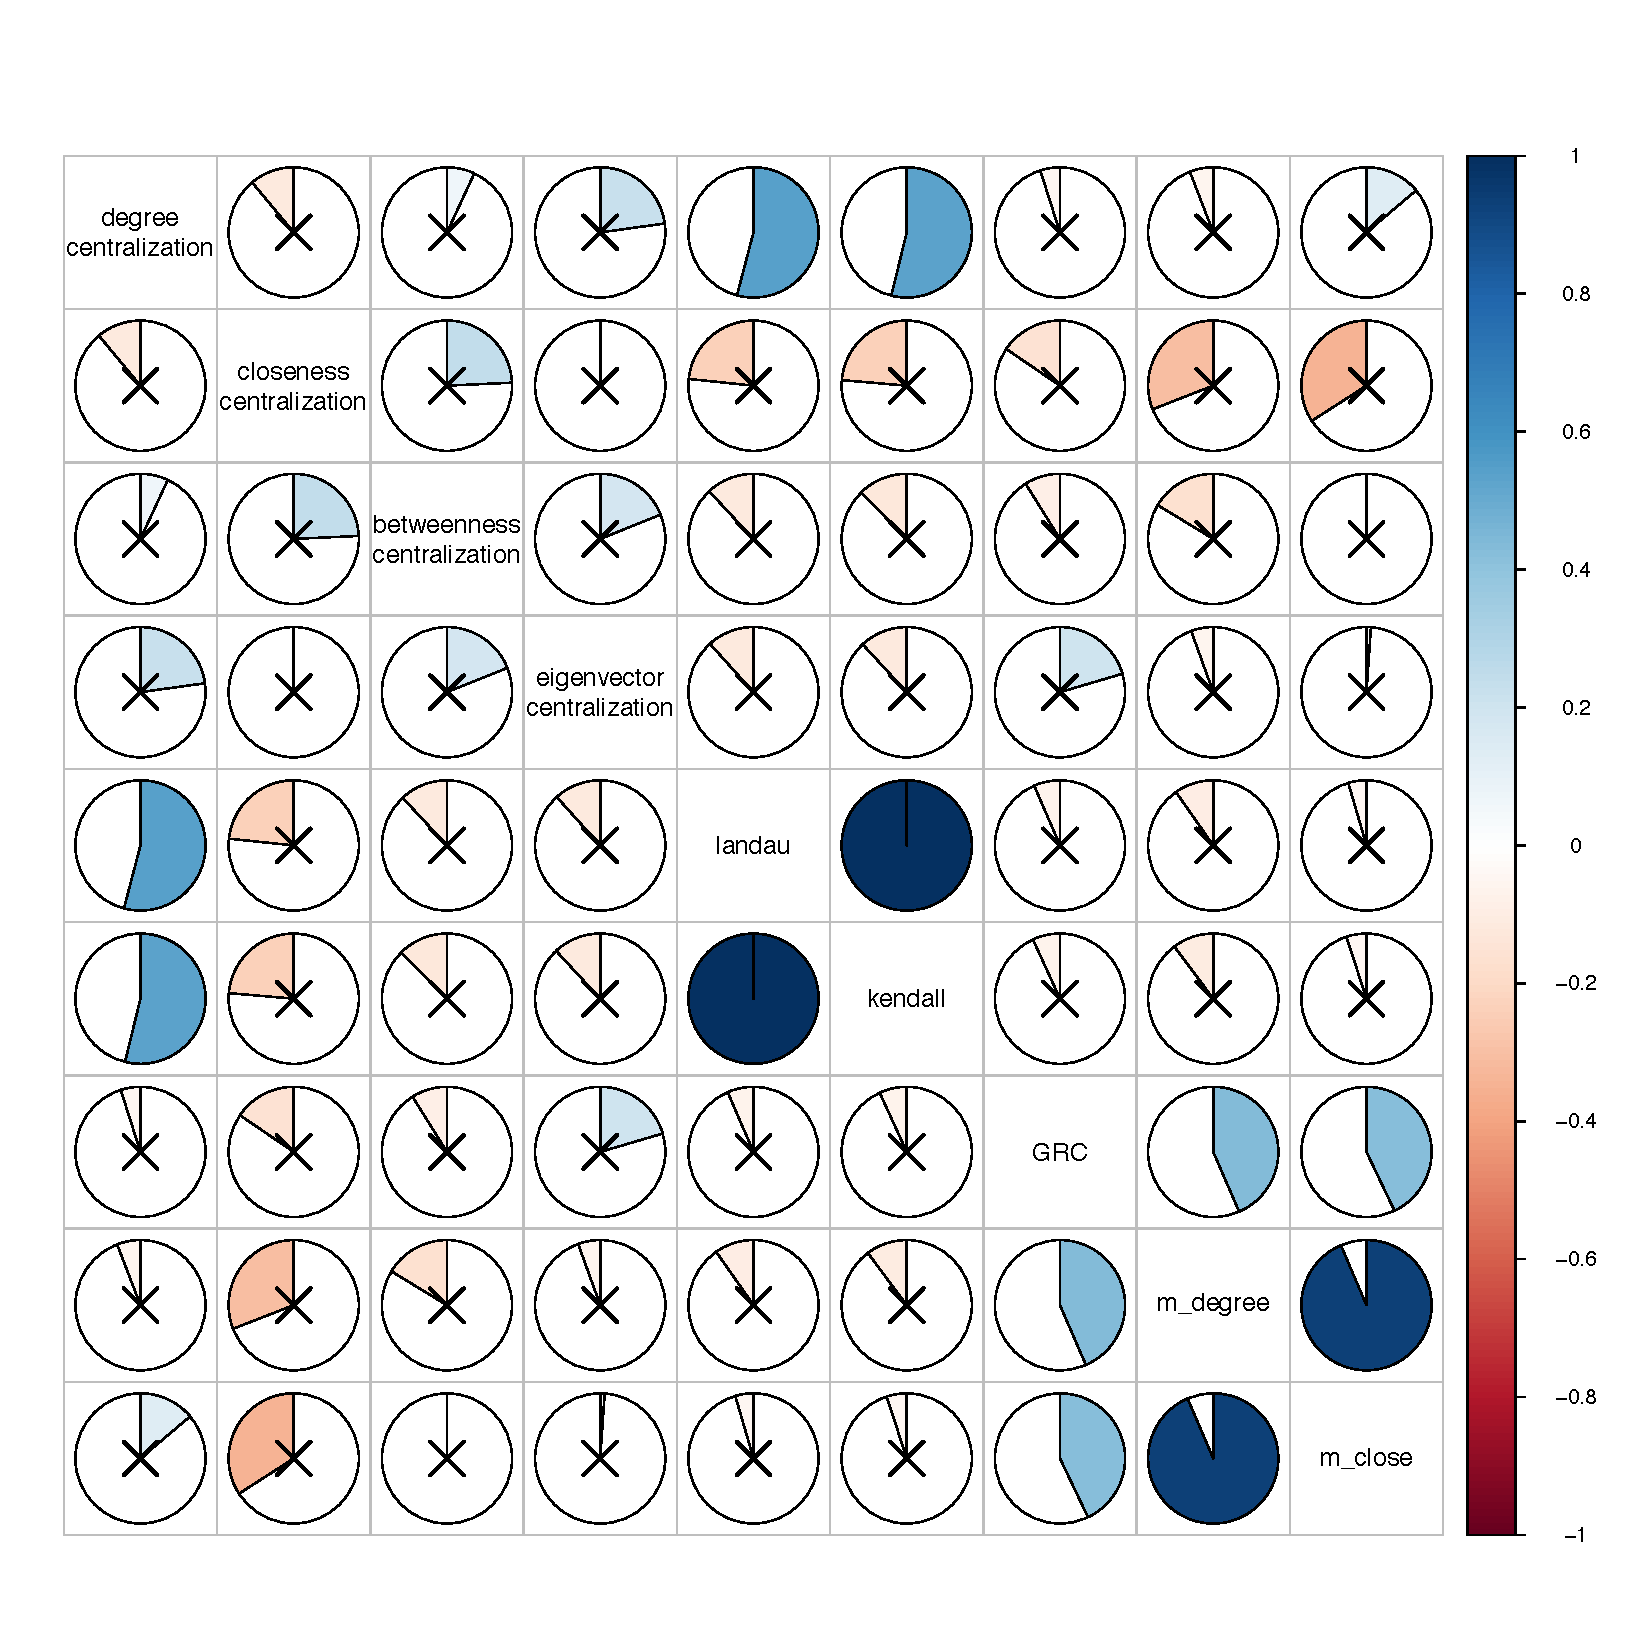
\includegraphics[width = 0.98\textwidth]{./images/Global_Measure_Correlations_with_Tests.pdf}
\end{center}
\end{figure}

Perhaps surprisingly, most of the rest of the correlations depicted in Figure \ref{fig:measure correlations} are relatively small and statistically insignificant, indicating that if all of these measures are valid, they are likely capturing different dimensions of hierarchy in a network. This finding suggests that either there are multiple dimensions to hierarchy in a network \cite{Corominas-Murtra2013}, some of these measures do not measure hierarchy, or some combination of both. To investigate this finding further, we perform several statistical and qualitative comparisons between these measures in Section \ref{sec:analysis}.
	
\section{Data}
\label{sec:data}
The data used in this study comprise 136 social networks, collected from three primary sources. The first of these is a set of seventeen email communication networks among department managers in North Carolina county governments. These data were collected as part of a field experiment described in Ben Aaron et al. (forthcoming), and comprise all department manager to department manager email communications over a three month period in 2013. In total, these networks include 17,863 emails sent between 362 department managers. The second set of networks record cosponsorship patterns in the United States Senate between 1973 and 2009. There are a total of eighteen networks, each recording the number of times Senator $i$ cosponsors (officially records support for) a piece of legislation sponsored by (introduced by) legislator $j$ during a two year session of Congress. The third primary source from which we obtain network data is the UCI-Net online network data repository\footnote{Data are freely available online here: \href{https://sites.google.com/site/ucinetsoftware/datasets}{https://sites.google.com/site/ucinetsoftware/datasets}}. We were able to obtain a total of 101 network datasets from this website, comprising a wide range of social, communication, and economic networks. Links to source data, and references for all networks used in this study will be made available in an appendix\footnote{We did not had time to compile this appendix before the end of the semester, but it will be included in the fina version of the paper.}.

Theoretically, we might expect different types of networks (social, information, biological, etc.) to display distinct relational structures, and perhaps exhibit common hierarchical structures. We therefore decided to hand code each of the 136 networks in our sample into one of eight broad categories. Descriptive statistics for networks in each of these categories are provided in Table \ref{tab:descriptive stats by type}. We can see that most networks have between twenty five and forty nodes on average, with the notable exception being the cosponsorship networks, which average roughly one hundred nodes. Note that the networks classified as \emph{unknown} have yet to be categorized due to the difficulty in navigating the UCI-Net data archives, but will be classified into one of the eight categories before publication. 
%A list of references for the network datasets used in this study can be found in \ref{sec:dataset references}.

% latex table generated in R 3.2.2 by xtable 1.8-0 package
% Sun Dec  6 14:21:01 2015
\begin{table}[ht]
\centering
\caption{\label{tab:descriptive stats by type} Network Descriptive statistics for all 136 networks in our sample, aggregated by the network type. All columns are averages over networks of that type.}
\begin{tabular}{lrrrrr}
  \toprule
 \textbf{Type} & \textbf{\# of Networks} & \textbf{Nodes} & \textbf{Edges} & \textbf{Density} & \textbf{Clustering Coefficient} \\ 
  \midrule
  \emph{communication} & 20 & 25.40 & 1764.25 & 2.87 & 0.55 \\ 
  \emph{cosponsorship} & 18 & 101.22 & 13358.89 & 1.32 & 0.79 \\ 
  \emph{co-membership} & 2 & 21.50 & 22.50 & 0.05 & 0.07 \\ 
  \emph{interaction} & 40 & 23.07 & 1944.95 & 1.99 & 0.59 \\ 
  \emph{unknown} & 33 & 38.70 & 445.36 & 0.38 & 0.43 \\ 
  \emph{friendship} & 6 & 29.83 & 92.00 & 0.12 & 0.35 \\ 
  \emph{affect} & 11 & 17.64 & 95.18 & 0.32 & 0.33 \\ 
  \emph{terrorism} & 1 & 63.00 & 308.00 & 0.08 & 0.36 \\ 
  \emph{trade} & 5 & 24.00 & 285.60 & 0.52 & 0.73 \\ 
   \bottomrule
\end{tabular}
\end{table}

% Before fitting any of the hierarchy measures on these real datasets, we want to make sure that the measures are invariant to the size of the network. We simulate $7500$ Barbasi-Albert (BA), $6000$ Tree-Structured (TR), and $4500$ Erdos-Renyi (ER) datasets, where one third of each type has $50$ nodes, a third has $200$, and the last third has $500$. We are also curious to see how the hierarchy measures perform while altering the parameters of these datasets. For the BA datasets, we set the preferential treatment parameter to $p=0.5, 1, 2, 5, 10$. We set the number of children parameter in the TR datasets to be $c=2, 5, 10, 50$, and the probability of forming and edge in the ER datasets to $d=0.05, 0.1, 0.2$. Figures can be found in Appendix C, which illustrate our findings. For the BA networks, we notice that Kendall and Landau's measures do not change as $p$ increases. We note that all other measures except for degree and closeness decrease as $p$ increases. For TR networks,  
	
% Among the network datasets we are exploring, they are already or mostly in usable format. As we're navigating through our theoretical conception of hierarchy in network, we are ruling out the use of the karate club, dolphin, football, etc. datasets because we want to be able to analyze datasets where the networks are more interesting or theoretically-relevant. In this way, there are a couple of systems that might be useful. The first is a network of cooperation among militant groups, which encompasses joint exercises, mergers, and splits among militant groups: http://web.stanford.edu/group/mappingmilitants/cgi-bin/. This may interesting for us for a few reasons: (1) there is no de jure hierarchical structure (i.e., no formally-recognized chain of command or sovereignty); (2) militant groups face a classic collective action problem, and thus we can expect the dynamics Mann describes to hold; and (3) most theories of conflict would predict no hierarchy to occur in this system. An interesting system to compare this to would be military actions in Vietnam: http://tinyurl.com/pwofooy. The nodes here would be military units, and the edges are participation in the same battle. Of course, the main issue with this dataset is that it's undirected, which we've noted may be difficult to conceptualize within a hierarchy framework. We're focusing on conflict datasets because many of the theoretical definitions define hierarchy as essentially about outcomes—i.e., the ability of particular nodes to control the actions and behaviors of subordinate nodes.
%
%  We may also use manager network data where each organization has a ``county manager" who is theoretically in charge of the rest of the actors, providing an opportunity to determine if the methods we employ capture a plausible hierarchical structure. We are still exploring this and other datasets though.





\section{Analysis}
\label{sec:analysis}


\subsection{Principal Components Analysis}
In order to find patterns in the various measures of hierarchy presented above, we rely on Principal Components Analysis (PCA). PCA is a dimension reduction technique commonly used in the social sciences. This works by finding the eigenvalues and eigenvectors of a set of variables, such that the components identified by the model maximize the variance accounted for. For the purposes of this analysis, we have 11 hierarchy measures calculated across the 136 networks described above. PCA allows us to detect the patterns behind this 11-dimension data, and constructs principal components such that most of the variance in the 11 dimension problem can be accounted by a fewer number of components.

Of course, there will be as many principal components as there are dimensions in the original data. PCA component eigenvalues are illustrated in Figure \ref{fig:PCA variacnes}. As is clear from this figure, while there are nominally 11 principal components, a vast majority of the variance present in the original problem is captured by the first four principal components. This four dimensional problem is much easier to interpret than the original 11D problem. A graphical comparison of components one and two is provided in Figure \ref{fig:1 and 2}. A graphical comparison of components one and three is provided in Figure \ref{fig:1 and 3}. A graphical comparison of components two and three is provided in Figure \ref{fig:2 and 3}. A graphical comparison of components one and four, two and four, and three and four are included in Figure \ref{fig:1 and 4}, Figure \ref{fig:2 and 4}, and Figure \ref{fig:3 and 4}, respectively.

\begin{table}[!htbp] \centering 
  \caption{\label{tab: PCA rotation} PCA Rotation for Components with Eigenvalues above 1} 
  \label{} 
\begin{tabular}{@{\extracolsep{5pt}} lcccc} 
\\[-1.8ex]\hline \\[-1.8ex] 
 & P.C. 1 & P.C. 2 & P.C. 3 & P.C. 4 \\ 
\hline \\[-1.8ex] 
Degree Centralization & $$-$0.017$ & $0.062$ & $$-$0.522$ & $0.222$ \\ 
Closeness Centralization & $$-$0.130$ & $$-$0.056$ & $$-$0.606$ & $$-$0.107$ \\ 
Betweenness Centralization & $$-$0.009$ & $0.437$ & $$-$0.292$ & $0.387$ \\ 
Eigenvector Centralization & $0.166$ & $0.040$ & $$-$0.239$ & $0.466$ \\ 
Landau's $h$ & $0.130$ & $0.454$ & $$-$0.126$ & $$-$0.481$ \\ 
Kendall's $K$ & $0.171$ & $0.506$ & $$-$0.098$ & $$-$0.395$ \\ 
GRC & $0.501$ & $$-$0.109$ & $$-$0.085$ & $$-$0.088$ \\ 
$m$-closeness & $0.539$ & $0.011$ & $0.045$ & $0.151$ \\ 
$m$-degree & $0.538$ & $$-$0.036$ & $0.087$ & $0.044$ \\ 
Krackhardt & $$-$0.055$ & $$-$0.408$ & $$-$0.346$ & $$-$0.370$ \\ 
Triangle Transitivity & $0.273$ & $$-$0.397$ & $$-$0.237$ & $$-$0.127$ \\ 
\hline \\[-1.8ex] 
\end{tabular} 
\end{table} 

Table \ref{tab: PCA rotation} presents the rotations, or factor loadings, which describe to what extent the original variable relates to the principal components. The first principal component, which accounts for 27.9\% of the variance, is most highly correlated with M--Reach Degree, M--Reach Closeness, and GRC. It is not surprising that these three measures load together, as GRC relies on M--Reach Closeness, which in turn relies on M--Reach Degree. As discussed in the description of the measures, this family of hierarchy measures describes how many nodes in a dominance network can be reached from a given node. In other words, these measures describe a type of hierarchy in which diffusion of authority is recognized by higher values. This corresponds closely to Mann's ``diffusion'' type described in the introduction; a type of power that varies according to how many subordinates can be immediately reached by a dominant actor.

Second, the third principal component is heavily loaded on degree and closeness centrality. As discussed in the analytical measures of hierarchy section, the former measures the number of connections for a given node, while the latter measures how easy it is to reach each node in the network from a given node. Returning to Mann's typology, this seems to measure a distinct concept from his two dimensions of hierarchy: diffusion (described by the first principal component) and authoritative. Instead, it seems to measure the extensiveness of a hierarchy. In other words, we could expect that networks which have a higher value on principal component 3 to have a deeper and more extensive hierarchical system, irrespective of the type of hierarchy they represent.

Finally, principal components 2 and 4 eschew a clear explanation and mapping on to Mann's typology. Components 2 and 4 are similar in that landau and kendall load about evenly between the two. Component 2 is more heavily loaded on Krackhardt and triangle transitivity, whereas component 4 is loaded heavily on Eigenvector centrality. Landau's h and Kendall's K are indicative of Mann's authoritative type of power, in that each measures the tree-ness of a network, with the highest value representing a perfect linear hierarchy. In social terms, this could be understood as a military type of hierarchy, where there are clear and rigid layers of authority. 

Component 2 loads more heavily on Krackhardt's hierarchy score and Triangle Transitivity. The former measures the extent that dyads are not reciprocal, while the latter has a very substantively similar interpretation to Landau's h and Kendall's K, because it was intended to be an improvement on those two measures. The concept of unreciprocated dyadic relationships matches closely onto Mann's conception of authoritative hierarchies, as these are clear dominant--subordinate relationships. Therefore, we argue that component 2 most closely maps to the authoritative type of hierarchy discussed by Mann.

Component 4 differs from Component 2 in that it loads heavily on eigenvector centralization, rather than triangle transitivity or Krackhardt's hierarchy score. Eigenvector centralization describes how well a node is connected to other well--connected nodes. A network with a high degree of eigenvector centralization is one in which a small coterie of well--connected nodes, exhibit control over a system. This is a slight deviation from the authoritative power type described by Mann. To put this into social terms, while Component 4 would describe a military system, Component 2 might describe an oligarchical system, which is comprised of both explicit dominant--subordinate relationships (captured by Kendall's K and Landau's h), but a group of individuals at the top, rather than a perfect tree which extends from the lowest rung to the highest rung.

\begin{figure}
\begin{center}
	\caption{\label{fig:PCA variacnes} Eigenvalues for 9 largest principle components in our analysis indicate that we should examine the first three components, which all have eigenvalues greater than one.}
		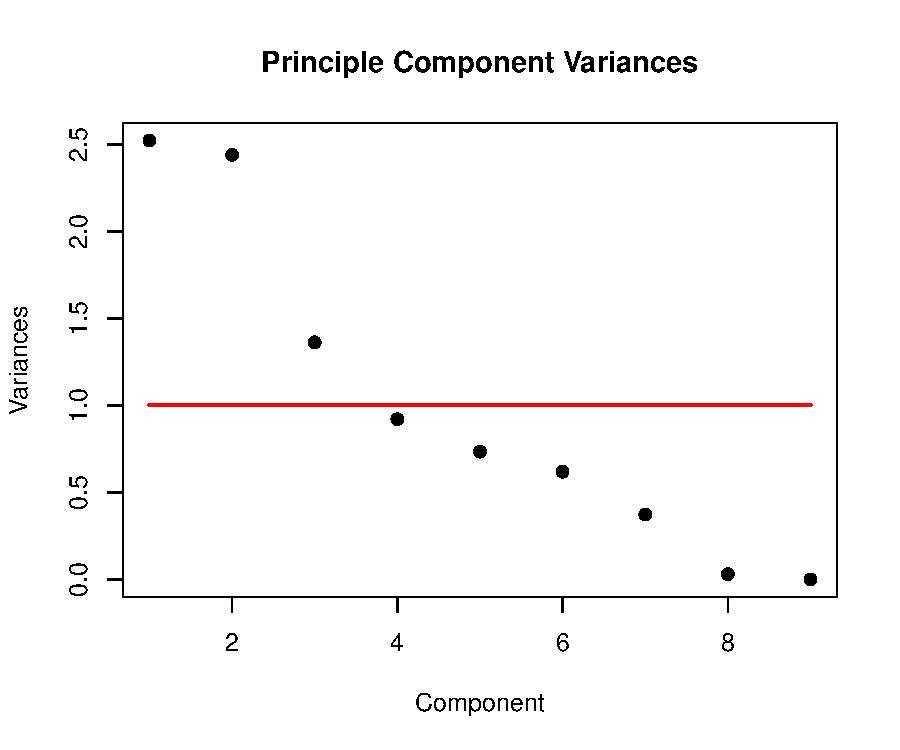
\includegraphics[width = 0.5\textwidth]{./images/Observed_PCA_Component_Varinces.pdf}
\end{center}
\end{figure}

\begin{figure}
\begin{center}
	\caption{\label{fig:1 and 2} Principle components plot for components one and two.}
		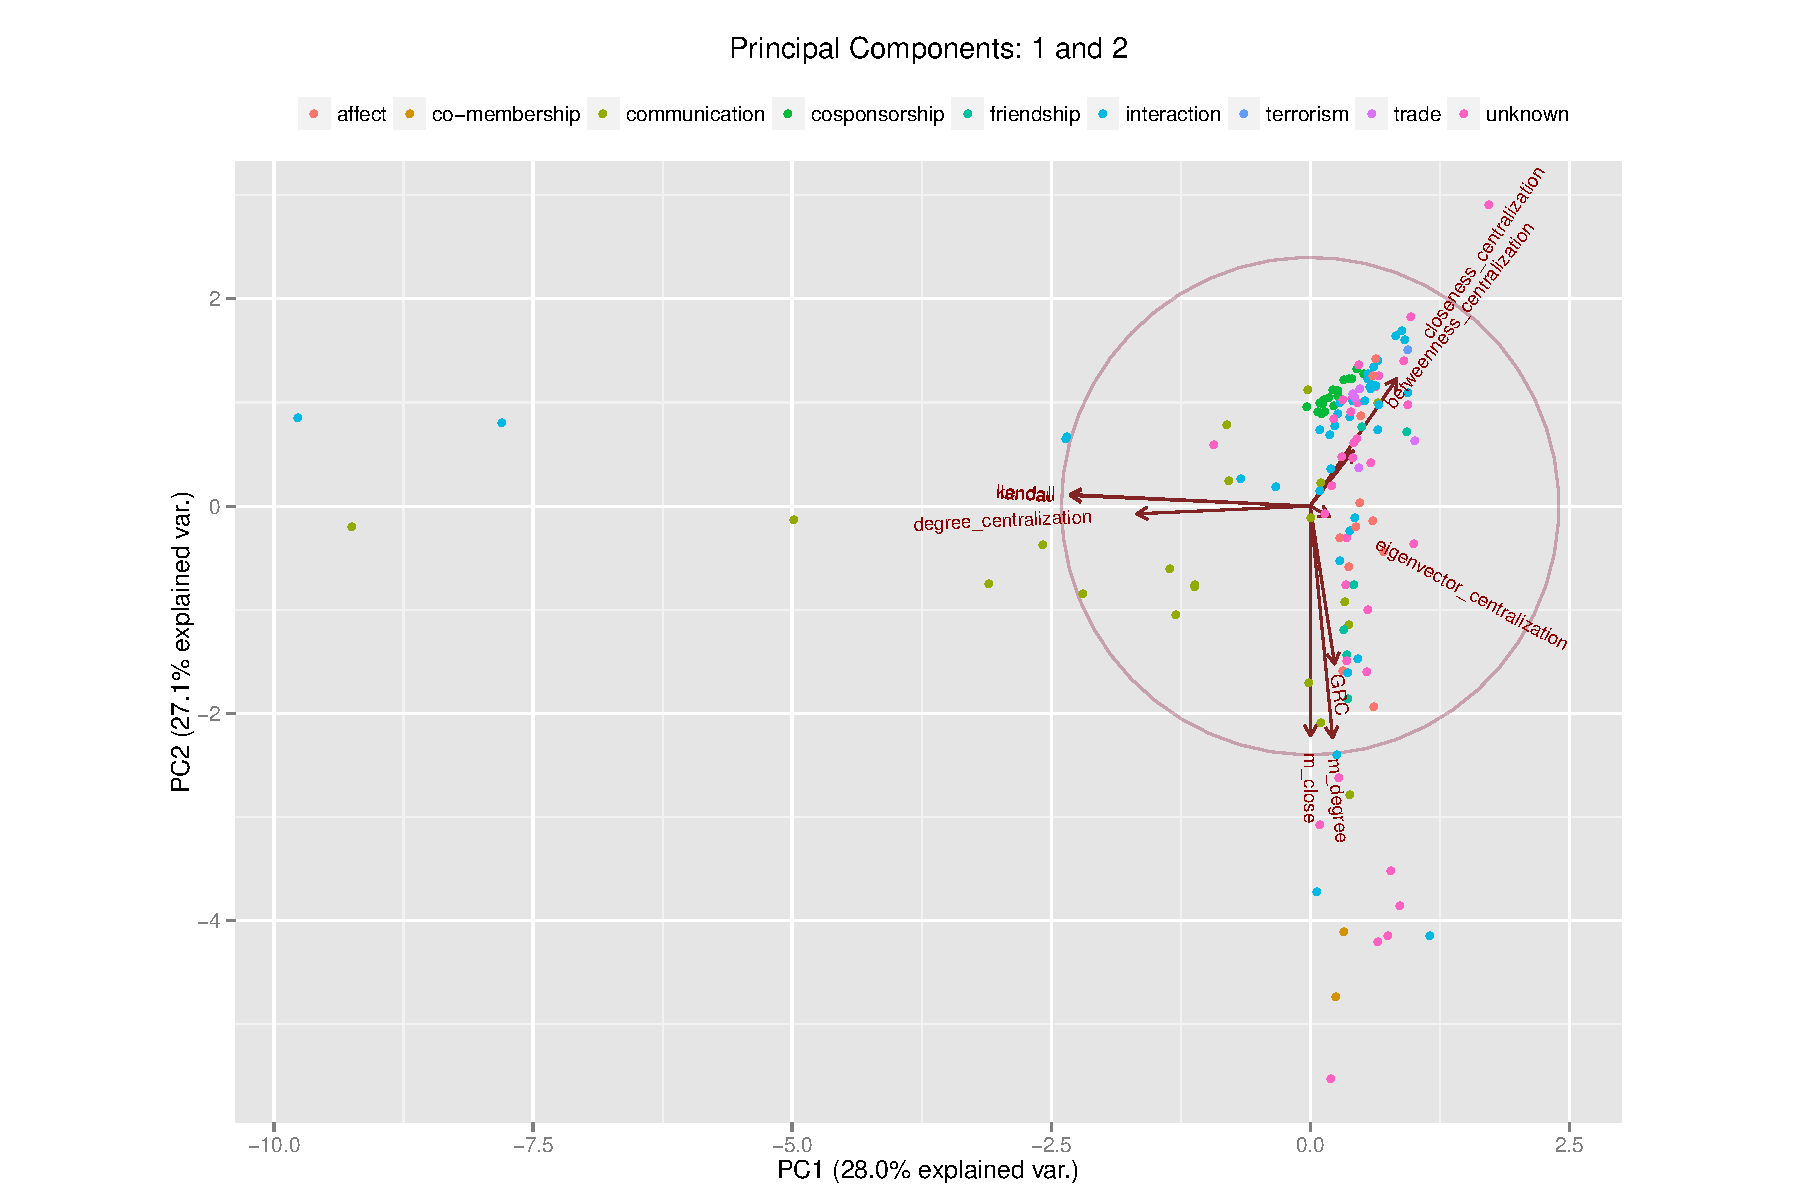
\includegraphics[width = 0.98\textwidth]{./images/Observed_PCA_Components1_2.pdf}
\end{center}
\end{figure}



% \subsection{Simulation Study}
% \label{sec:simulated figures}
%
% \begin{figure}
% 	\begin{center}
% 		\caption{\label{fig::Simulated Parameters} All figures show the average normalized global measure (denoted by the symbol in the bottom right key) by parameter value. The top left plot is for BA networks. The top right is for TR netwroks. The bottom left is for ER networks.}
% 		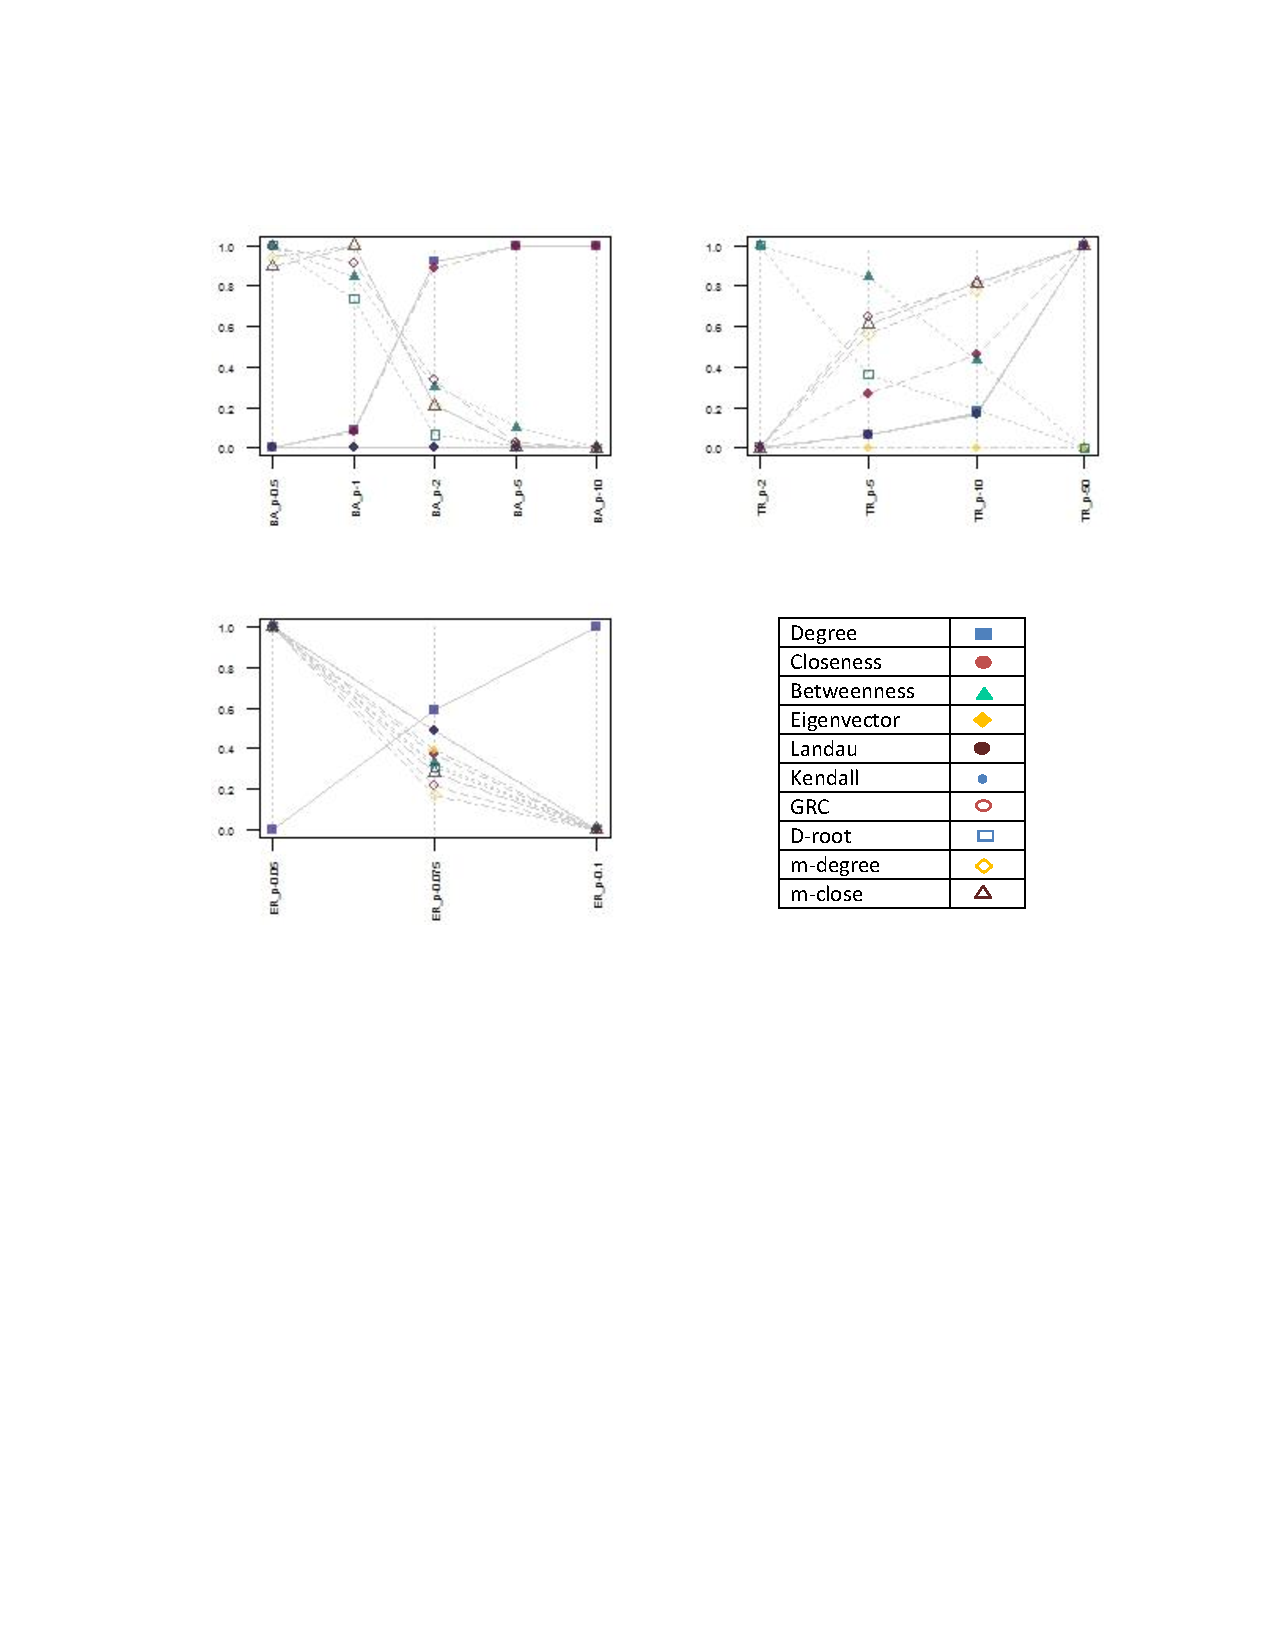
\includegraphics[width = 0.70\textwidth]{./images/Norm_Pars.pdf}
% 	\end{center}
% \end{figure}
%
% \begin{figure}
% 	\begin{center}
% 	\caption{\label{fig::Simulated Size} All figures show the average normalized global measure (denoted by the symbol in the bottom right key) by pnumber of nodes. The top left plot is for BA networks. The top right is for TR netwroks. The bottom left is for ER networks.}
% 	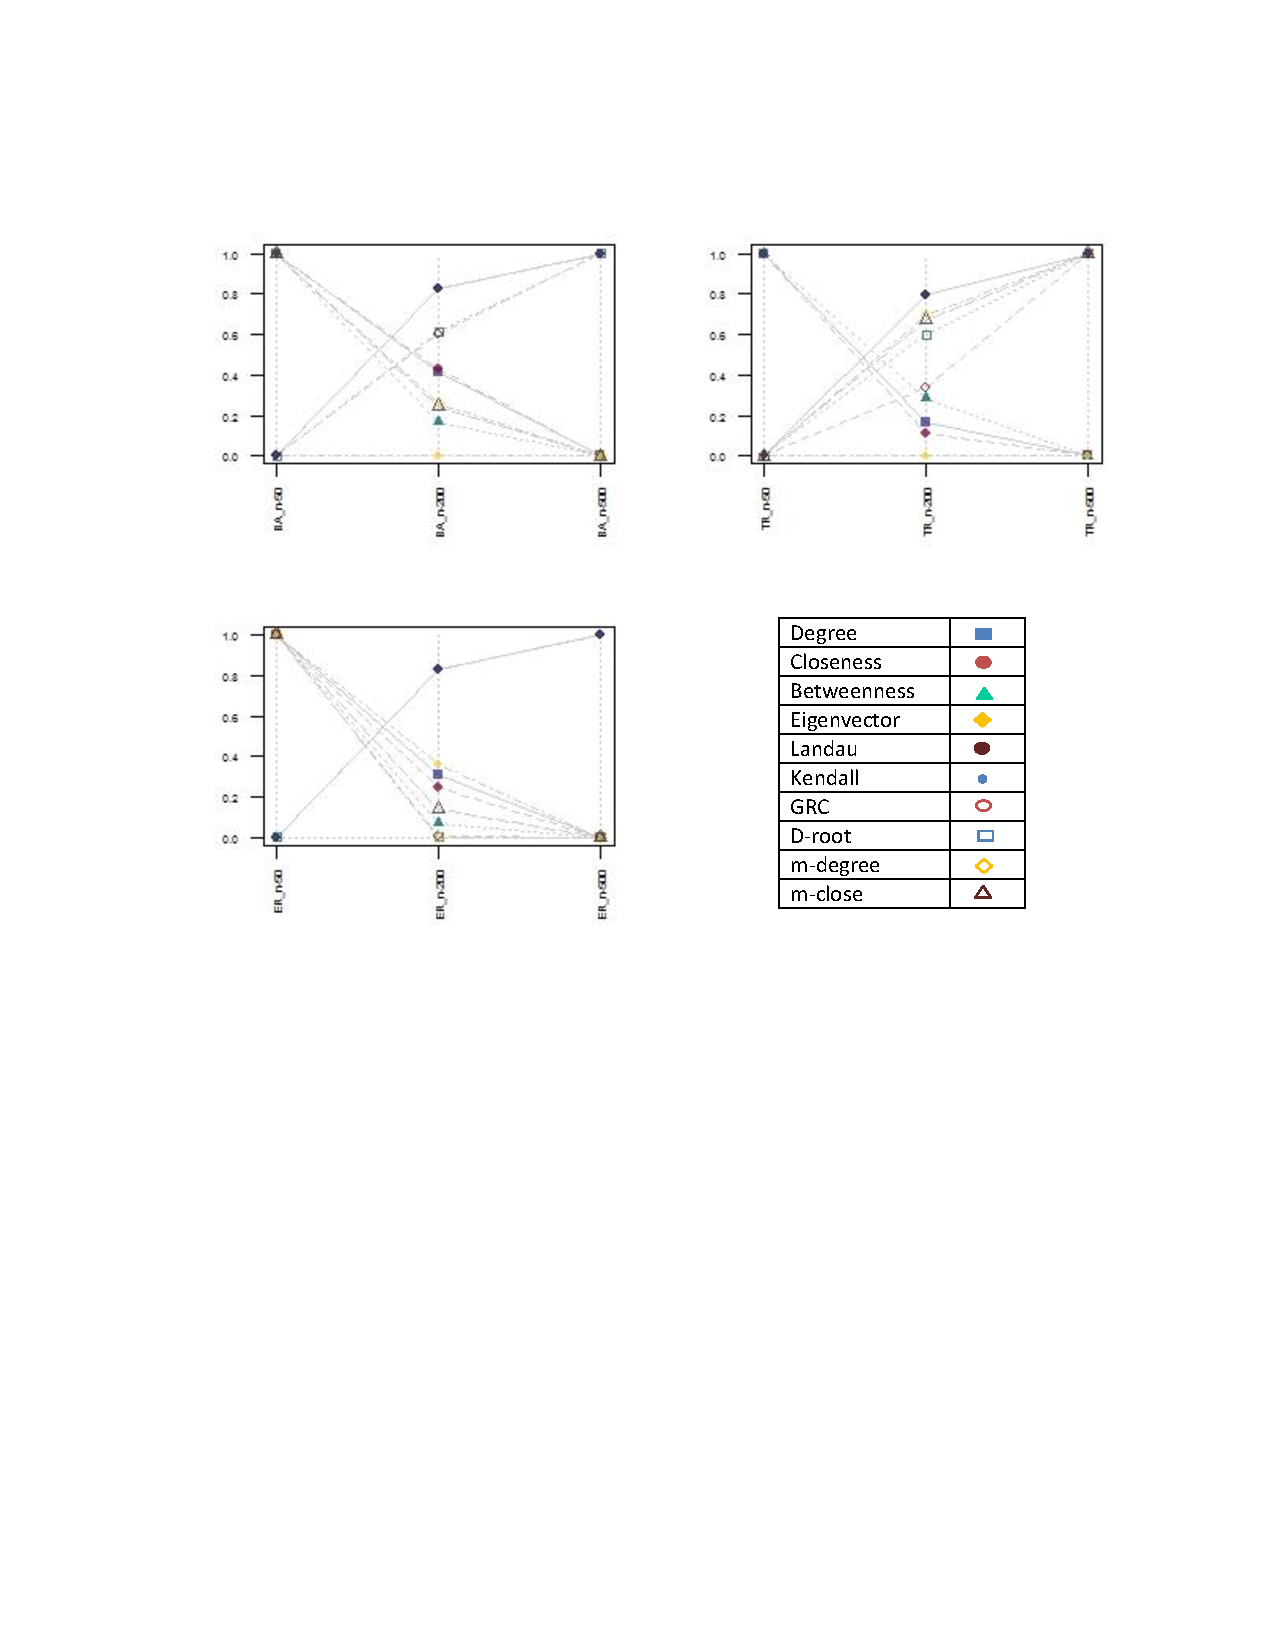
\includegraphics[width = 0.70\textwidth]{./images/Norm_Size.pdf}
% 	\end{center}
% \end{figure}


% latex table generated in R 3.2.2 by xtable 1.8-0 package
% Fri Dec 11 16:43:36 2015

\subsection{Ground Truth Rankings}

Seven of the twelve measures of hierarchy discussed above have a local analogue to the global measures we discuss in the previous sections.  To further understand the relative performance of these seven measures, we compare their ability to correctly recover the rank of the highest ranking manager in the seventeen county government email networks we analyze. Using our ground-truth knowledge of who should be be ranked at the top of the organizational hierarchy, Table \ref{tab:average local rankings} presents average ranking scores for each of the measures. These scores theoretically range between zero and one, with a score of one indicating that the measure ranks the county manager at the top of the hierarchy in every single county, and a score of zero indicating that the county manager was ranked at the bottom of the hierarchy in every single county. The measure with the best performance is closeness centrality (the local analogue to closeness centralization), which provided 82\% of optimal performance in ranking the county managers. This finding is not very surprising, because the county manager is the only member of the county government with incentives to interact with all of the other county managers directly. Generalized Reaching Centrality consistently provided the lowest performance across the board in this task, indicating it may not be a good measure for applications involving communication network data, but we generally see quite a bit of heterogeneity in the rankings across counties (see Figure \ref{fig:rankings each county}).  It is notable that many of the measures are able to accurately rank the county manager a high proportion of the time, indicating that they are at least partially capturing the concept of hierarchy in these networks. 

\begin{table}[ht]
\centering
\caption{\label{tab:average local rankings} Average Ranking index scores for each of the seven measures with a local analogue. A score closer to one indicates that a measure ranked the county manager in each county closer to the top of the hierarchy across the seventeen counties in our sample.}
\begin{tabular}{lr}
  \toprule
 & Average Rank Score \\ 
  \midrule
Degree Centrality & 0.75 \\ 
  Closeness Centrality & 0.82 \\ 
  Betweenness Centrality & 0.78 \\ 
  Eigenvector Centrality & 0.78 \\ 
  $m$-degree & 0.81 \\ 
  $m$-close & 0.63 \\ 
  GRC & 0.36 \\ 
   \bottomrule
\end{tabular}
\end{table}

One of the key issues with this approach is that we cannot compare four of the measures of hierarchy because they lack a local analogue. Therefore we cannot say whether closeness centralization is the best measure of hierarchy in organizational communication networks, because we lack a valid means of comparison. Also, as noted in the previous subsection, theory indicates that there are multiple dimensions to the concept of hierarchy, something that PCA confirms. 




% 	The analytical portion of the problem will be conducted in R, which is known by all members of the group. We will be using both statistical and mathematical methods of quantifying and/or measuring hierarchy. We will focus on methods that have already been developed, published, and implemented in R, or are can easily be implemented by one of the group members. If time permits, we may try to develop or suggest directions for future development of our own statistical models and/or mathematical measurements. Each member of the group will be responsible for at least one method.
%
% The statistical methods we will be looking into include hierarchical exponential graph models in the R package hergm. This package also includes hierarchical stochastic block models. Unlike fitting network data with exponential random graph models (ERGMs), hierarchical ERGMs focus on inducing local dependencies. Next, we will focus on latent space models, which can be fit in R using the latentnet package in the statnet suite of packages. For both the latent space and ERGM models, Bayesian inferential analysis can be conducted using the Bergm, VBLPCM, and lvm4net packages in R. We note that whenever fitting network data there is always the chance for computational timing and accuracy issues to come up. We have chosen a number of datasets for the purposes of capturing several types of hierarchies, but also so that we may have a few that are easily fit in R. Lastly, we will focus on mathematical measures of hierarchy. These measures primarily stem from graph theory, and can be easily programed by ourselves in R. The measurements include the Global Reach Centrality (GRC), Triangle Transitivity, Kendall's K, and Landau's lambda.



\section{Conclusions}
Inferring and measuring the power dynamics underlying human social behavior is a fundamental problem for all social scientists. We began this paper by discussing the importance of networks in reaching a rigorous understand of social dynamics, and how the concept of power is inherently relational, and therefore ripe for a network--oriented approach. However, power can be a nebulous concept to define theoretically, let alone measure empirically. In order to guide our understanding of the latter, we discussed Michael Mann's typology of different types of hierarchy, and provided alternative definitions to guide researchers.

Second, we surveyed the wide variety of analytical measures currently employed by network researchers. While there are similarities, these measures clearly focus on different aspects of network structure, and, when applied, will lead the researcher to draw different inferences. While this variety is useful to the researcher who wishes to find the exact measure to apply to her specific problem, if the measure of choice is simply \emph{assumed} to be representative of hierarchy, this increases researcher degrees--of--freedom and could lead to uninformed applications that do not adequately square the theoretical concept in question with the analytical technique being used.

Third, as a first cut to parse these measures, we provided simulations that demonstrate how each measure reacts to changes in network features. %Are we stil doing this?! --Mitch%

Finally, we contrasted the measures performance on a wide variety of observed social networks. First, we applied PCA to reduce the dimensionality of the various hierarchy measures. From this, the following conclusions can be drawn: M--Reach Degree, M--Reach Closeness, and GRC measure a type of diffusion hierarchy where spread of information is critical to control; Degree and Closeness Centrality measures the extent, rather than specific type, of hierarchy; and the remaining measures map on to Mann's authoritative power type with one capturing rigid, tree--like hierarchies, and the other capturing authorative hierarchies where power is concentrated in an elite group. Second, for the measures where we could calculate a local score, we applied them to hierarchies with a clear power structure known to us outside of the network being measured. %Add a couple sentences about the conclusion for ground--truth here%

%\bibliographystyle{elsarticle-num}
\clearpage
\bibliography{library,AddCitesHere}


% these still need to be translated to BibTeX
%
% 	\bibitem{monks}
% 	Breiger, R., Boorman, S., and Arabie, P. (1975),
% 	``An algorithm for clustering relational data with applications to social network analysis and comparison with multidimensional scaling."
% 	\textit{Journal of Mathematical Psychology} 12.
%
% 	\bibitem{libi}
% 	Brozovsky, L. and Petricek, V. (2007),
% 	``Recommender system for online dating service."
% 	\textit{Proc. Znalosti} 29-40.
%
% 	\bibitem{docs}
% 	Coleman, J., Katz, E., and Menzel, H. (1957),
% 	``The diffusion of an innovation among physicians."
% 	\textit{Sociometry} 253-270.
%
% 	\bibitem{HS}
% 	Coleman, J. (1973),
% 	``Introduction to mathematical sociology."
% 	\textit{London Free Press Glencoe}.
%
%
% 	\bibitem{Res}
% 	Freeman, L., Webster, C., and Kirke, D. (1998),
% 	``Exploring social structure using dynamic three--dimensional color images."
% 	\textit{Social Networks} 20: 2, 109-118.
%
% 	\bibitem{friendster}
% 	Friendster network dataset - KONECT, May 2015.
%
% 	\bibitem{URV}
% 	Guimera, R., Danon, L., Diaz-Guilera, A., Giralt, F., and Arenas, A. (2003),
% 	``Self--similar community structure in a network of human interactions."
% 	\textit{Phys. Rev. E.} 68: 6.
%
% 	\bibitem{online}
% 	Gupte, M., Shankar, P., Li, J., Muthukrishnan, S., and Iftode, L. (2011),
% 	``Finding Hierarchy in Directed Online Social Networks."
% 	\textit{International World Wide Web Conference Committee (IW3C2)}.
%
% 	\bibitem{Digg}
% 	Hogg, T. and Lerman, K. (2012),
% 	``Social dynamics of Digg."
% 	\textit{EPJ Data Science} 1, 5.

%
% 	\bibitem{EU}
% 	Leskovec, J., Kleinber, J., and Faloutsos, C. (2007),
% 	``Graph Evolution: Densification and Shrinking Diameters."
% 	\textit{ACM Transactions on Knowledge Discovery from Data (ACM TKDD)} 1: 1.
%
% 	\bibitem{livejournal}
% 	Leskovec, J., Lang, K., Dasgupta, A., and Mahoney, M. (2009),
% 	``Community Structure in Large Networks: Natural Cluster Sizes and the Absence of Large Well-Defined Clusters."
% 	\textit{Internet Mathematics} 6: 1, 29-123.
%
% 	\bibitem{wiki}
% 	Leskovec, J., Huttenlocher, D., and Kleinberg, J. (2010),
% 	``Predicting Positive and Negative Links in Online Social Networks."
%
% 	\bibitem{linux}
% 	Linux kernel mailing list replies network dataset - KONECT, May 2015.
%
% 	\bibitem{Liu12}
% 	Liu, Y., Slotine, J., and Barab{\'a}si, A (2012),
% 	``Control centrality and hierarchical structure in complex networks."
% 	\textit{Plos ONE:} 7: 9.
%
%
% 	\bibitem{facebook}
% 	McAuley, J. and Leskovec, J. (2012),
% 	``Learning to Discover Social Circles in Ego Networks."	\textit{NIPS}.
%
% 	\bibitem{manufacturing}
% 	Michalski, R., Palus, S., and Kazienko, P. (2011),
% 	``Matching organizational structure and social network extracted from email communication."
% 	Lecture Notes in Business Information Processing: 87, 196-206.
%
% 	\bibitem{youtube}
% 	Mislove, A., Marcon, M., Gummadi, K., Druschel, P., and Bhattacharjee, B. (2007),
% 	``Measurement and analysis of online social networks."
% 	\textit{Proc. Internet Measurement Conference}.
% 	%
%
% 	\bibitem{AdHealth}
% 	Moody, J. (2001),
% 	``Peer influence groups: Identifying dense clusters in large networks."
% 	\textit{Social Networks} 23: 4, 261-283.
%
% 	\bibitem{irvine}
% 	Opsahl, T. and Panzarasa, P. (2009),
% 	``Clustering in weighted networks."
% 	\textit{Social Networks} 31: 2, 155-163.
%
% 	\bibitem{cite}
% 	Prosper loans network dataset - KONECT, May 2015.
%
% 	\bibitem{epinions}
% 	Richardson, M., Agrawal, R., and Domingos, P. (2003),
% 	``Trust Management for the Semantic Web." \textit{ISWC}.
%
% 	\bibitem{Taro}
% 	Schwimmer, E. (1973),
% 	``Exchange in the Social Structure of the Orokaiva: Traditional and Emergent Ideologies in the Northern District of Papua." \textit{St. Martin's Press}.
%
% 	\bibitem{pokec}
% 	Takac, L. and Zabovsky, M. (2012),
% 	``Data Analysis in Public Social Networks."
% 	International Scientific Conference \& International Workshop Present Day Trends of Innovations, Lomza, Poland.
%
% 	\bibitem{Dutch}
% 	Van de Bunt, G., Van Deuijn, M., and Snijders, T. (1999),
% 	``Friendship networks through time: An actor-oriented dynamic statistical network model."
% 	\textit{Computational and Mathematical Organization Theory} 5: 2, 167-192.
%
% 	\bibitem{sevies}
% 	Watts, D. and Strogatz, S. (1998),
% 	``Collective dynamics of `small world' networks."
% 	\textit{Nature} 393: 1, 440-442.
%
% 	\bibitem{wiki2}
% 	West, R., Paskov, H., Leskovec, J., and Potts, C. (2014),
% 	``Exploiting Social Network Structure for Person-to-Person Sentiment Analysis."
% 	\textit{Transactions of the Association for Computational Linguistics} 2: 297-310.
%
% \end{thebibliography}
% \bibitem must have the following form:
%   \bibitem{key}...
%

% \bibitem{}

% \end{thebibliography}

\clearpage
\appendix

\section{Additional Plots}
 \label{sec:PCA Plots}

\begin{figure}
\begin{center}
	\caption{\label{fig:1 and 3} Principle components plot for components one and three.}
		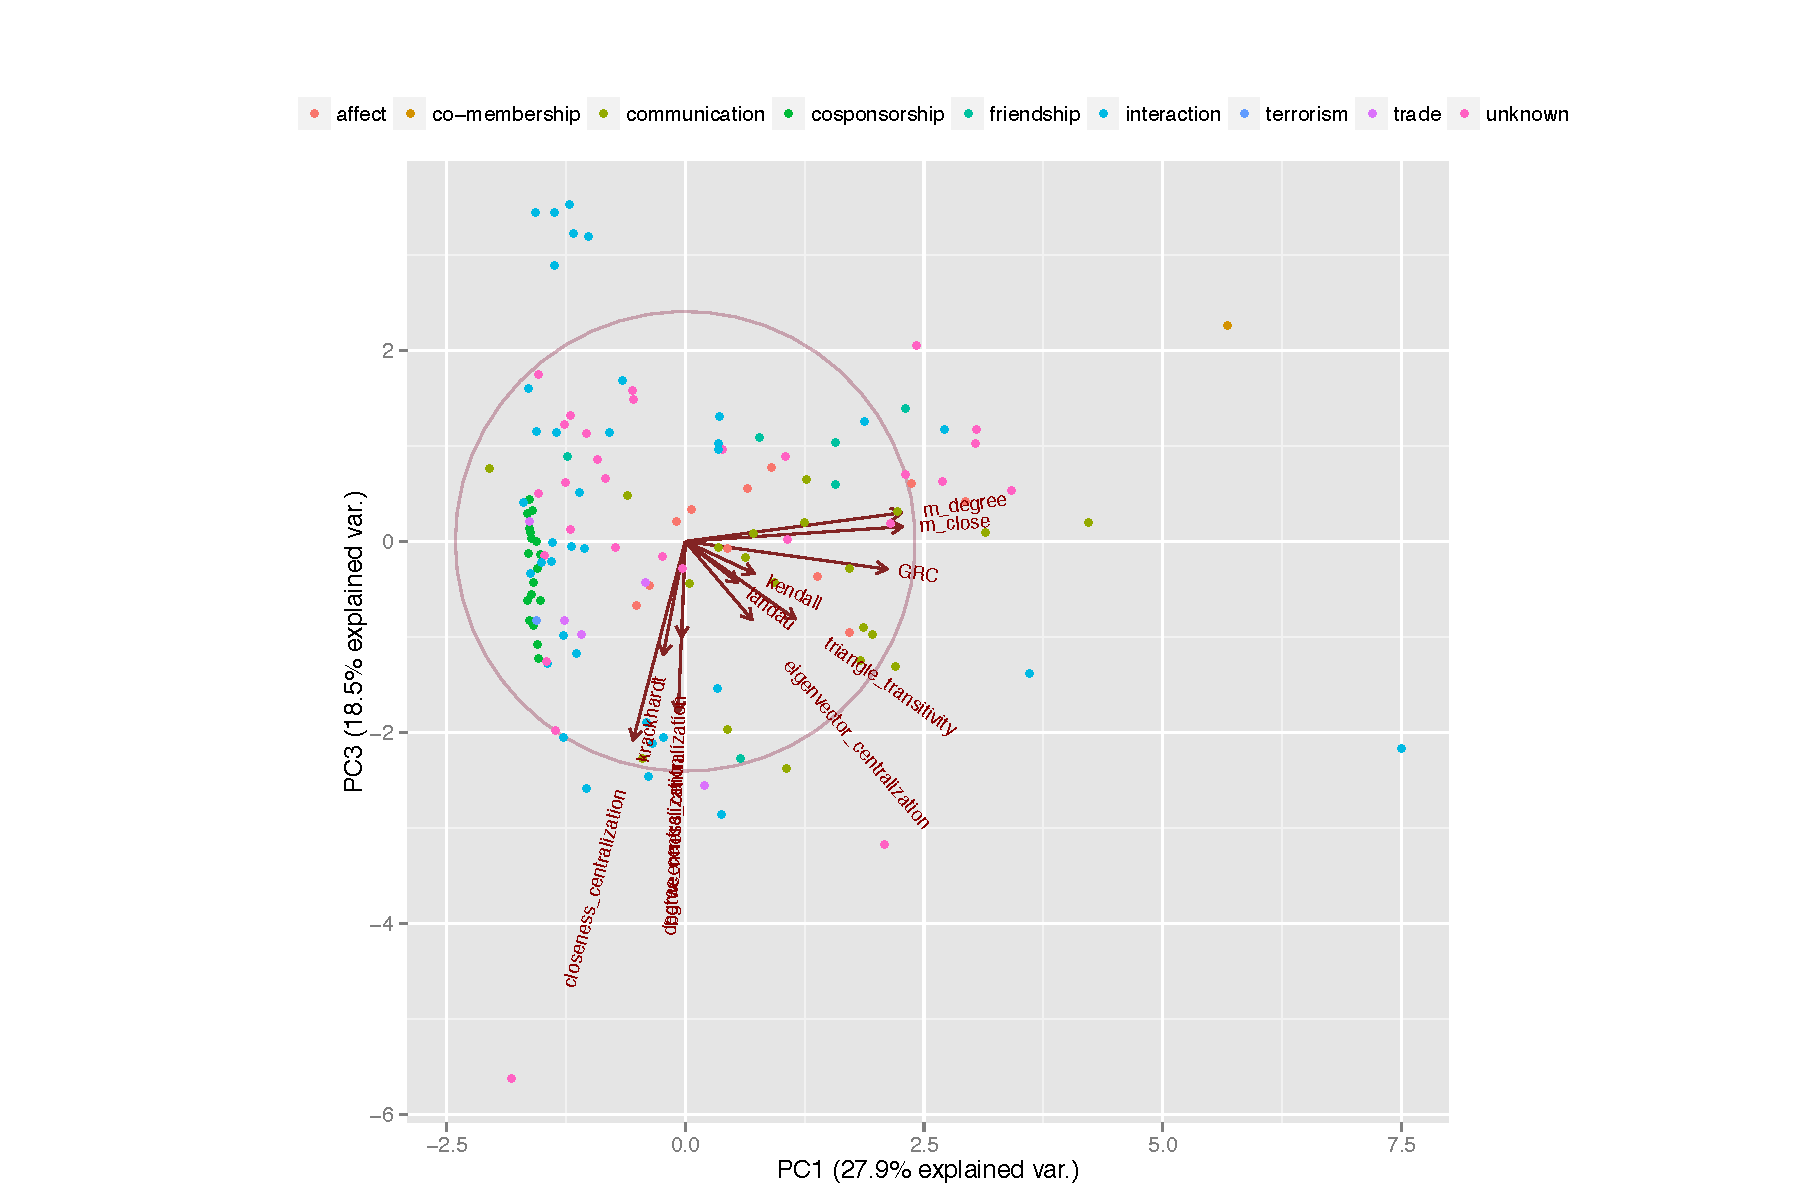
\includegraphics[width = 0.98\textwidth]{./images/Observed_PCA_Components1_3.pdf}
\end{center}
\end{figure}

\begin{figure}
\begin{center}
	\caption{\label{fig:1 and 4} Principle components plot for components one and four.}
		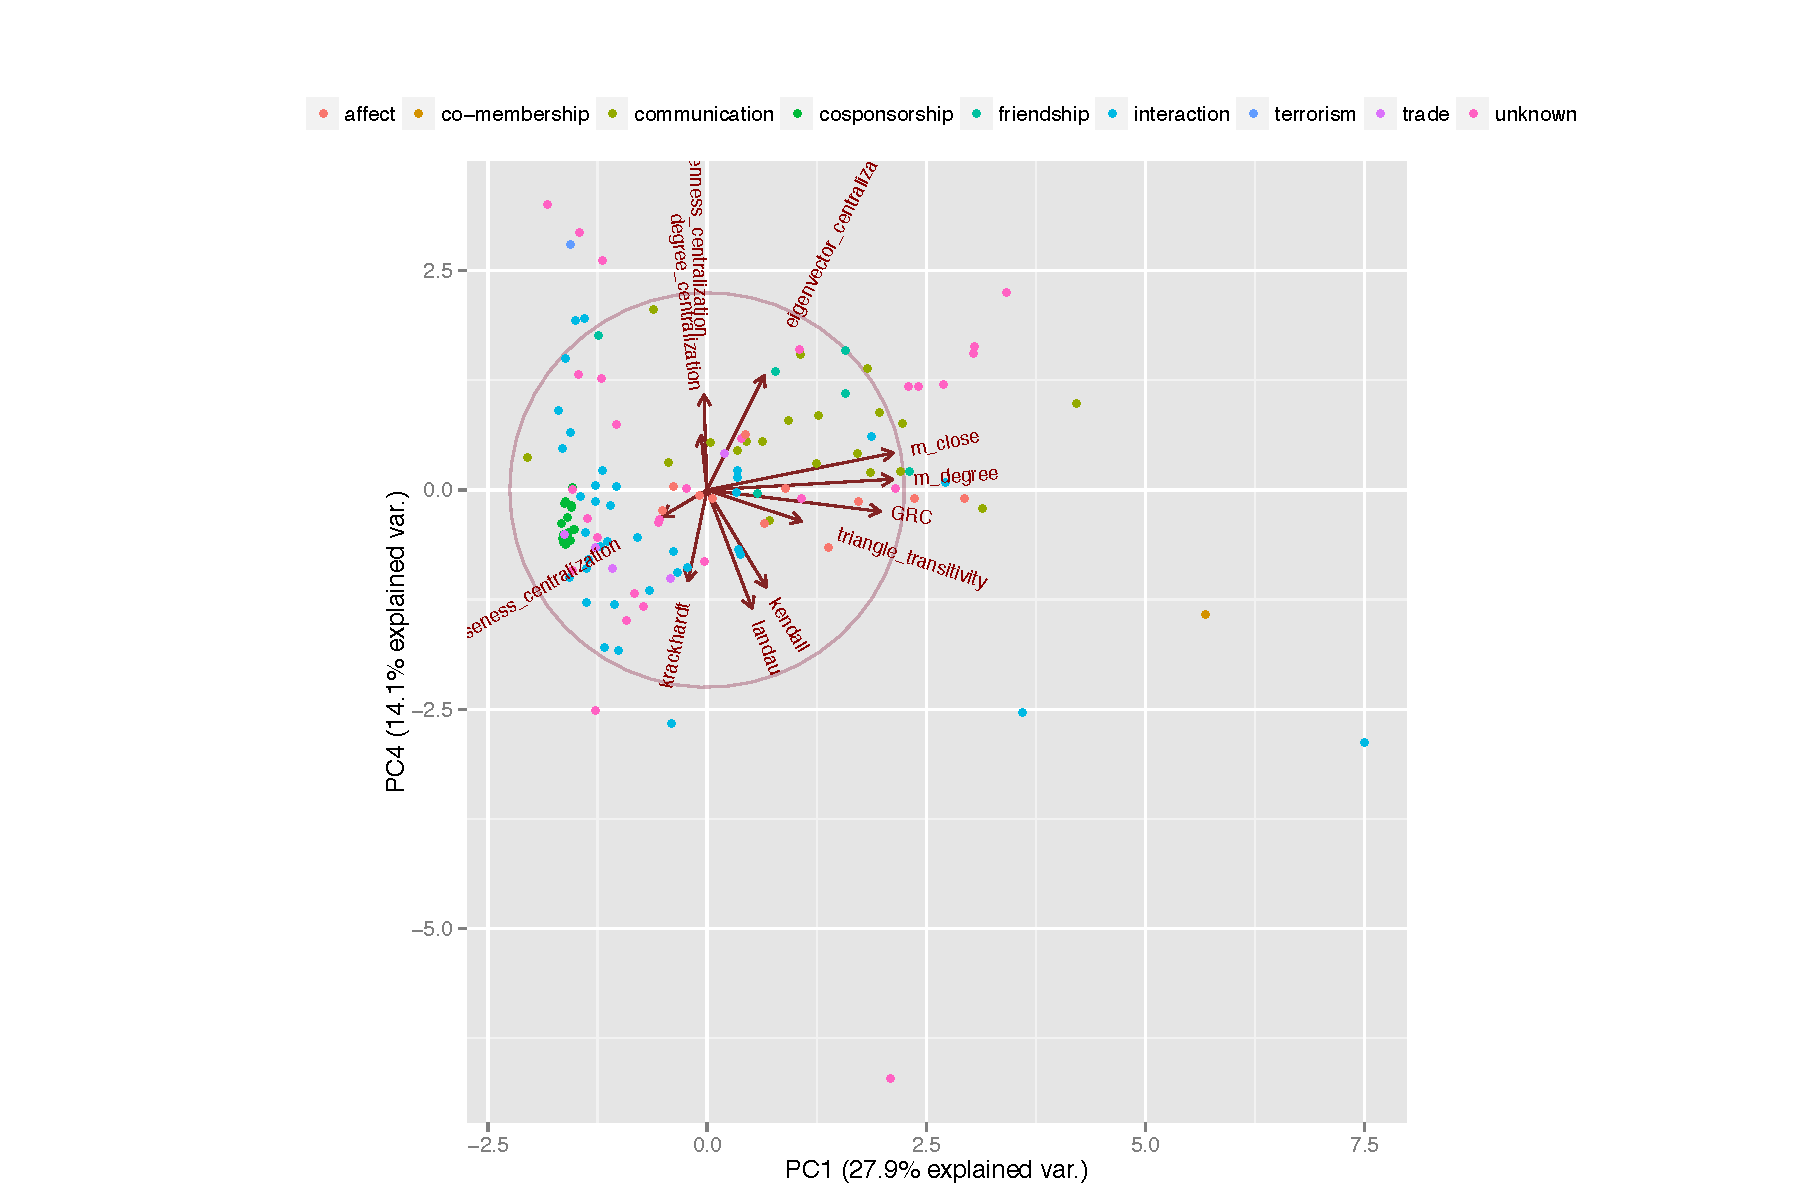
\includegraphics[width = 0.98\textwidth]{./images/Observed_PCA_Components1_4.pdf}
\end{center}
\end{figure}

\begin{figure}
\begin{center}
	\caption{\label{fig:2 and 3} Principle components plot for components two and three.}
		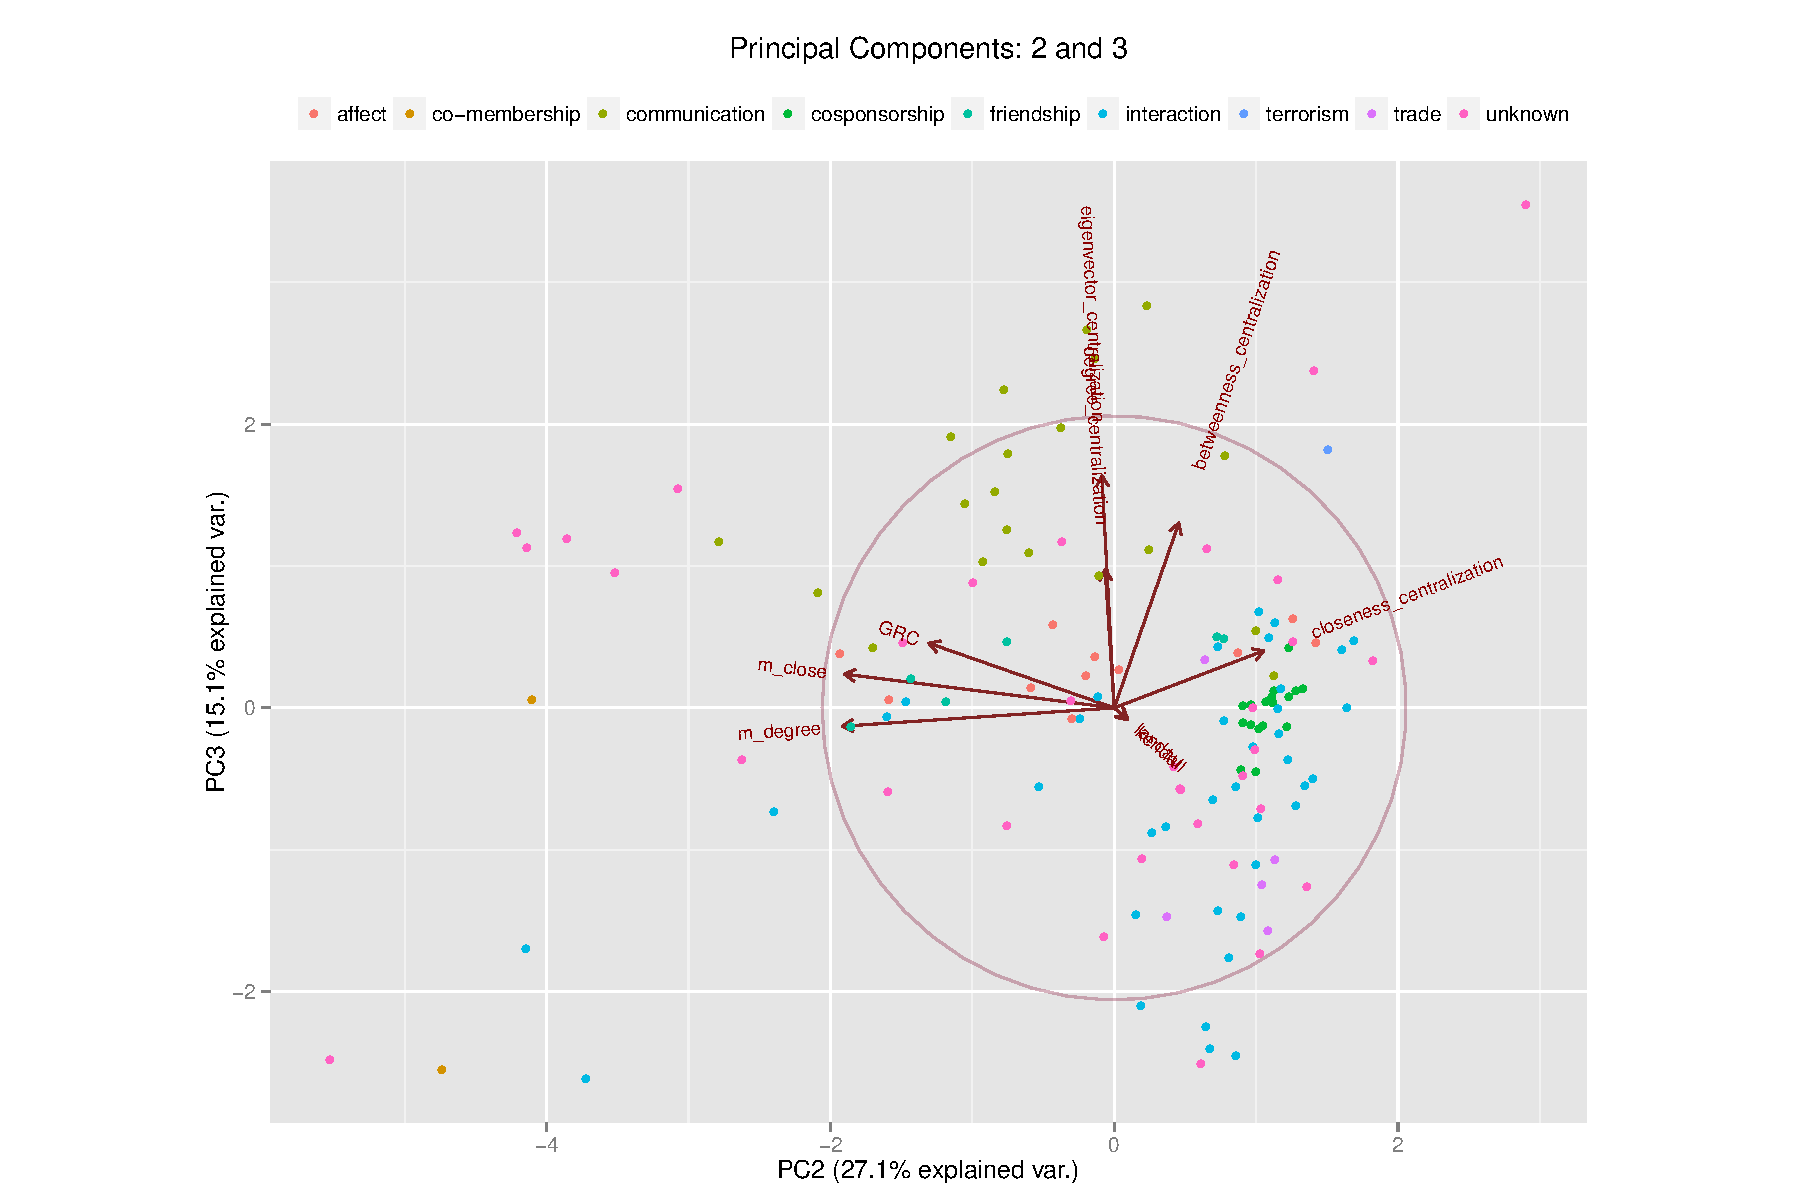
\includegraphics[width = 0.98\textwidth]{./images/Observed_PCA_Components2_3.pdf}
\end{center}
\end{figure}

\begin{figure}
\begin{center}
	\caption{\label{fig:2 and 4} Principle components plot for components two and four.}
		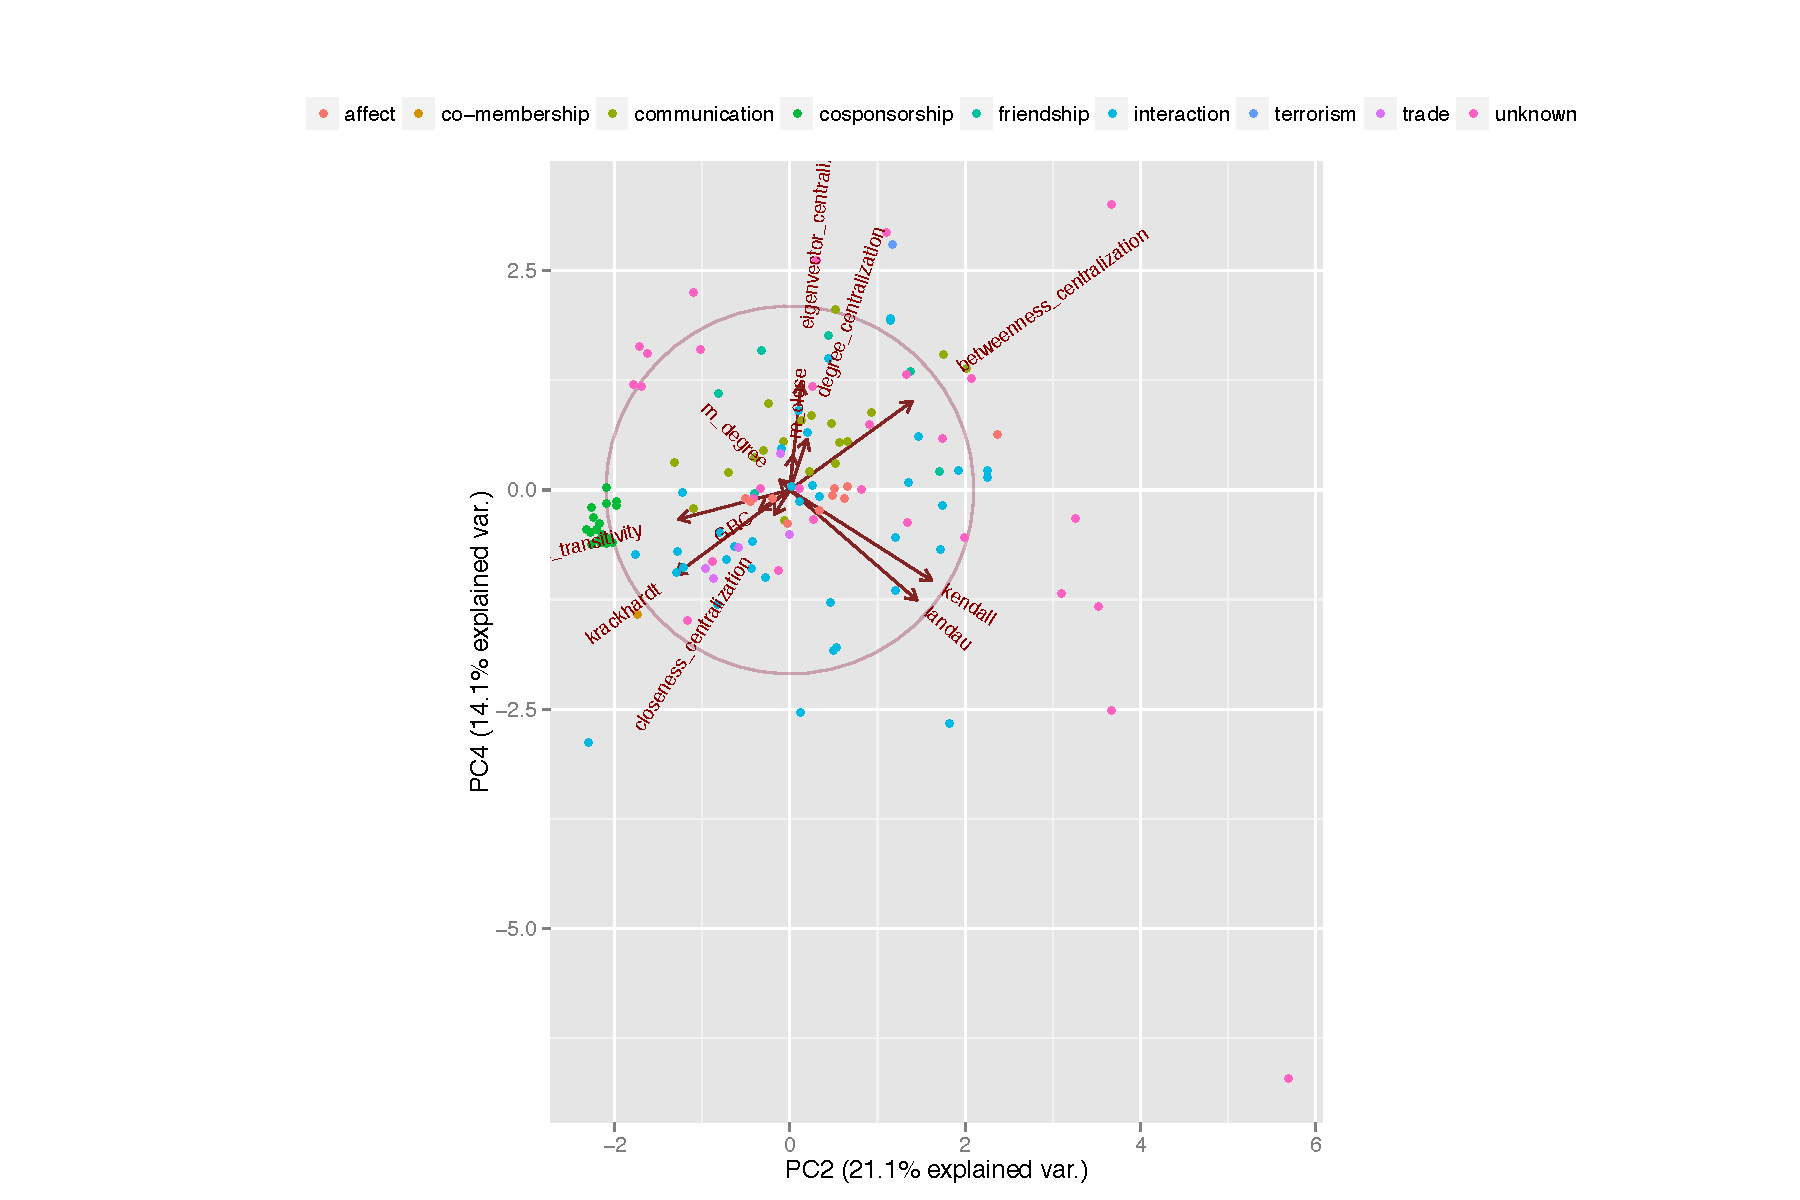
\includegraphics[width = 0.98\textwidth]{./images/Observed_PCA_Components2_4.pdf}
\end{center}
\end{figure}

\begin{figure}
\begin{center}
	\caption{\label{fig:3 and 4} Principle components plot for components three and four.}
		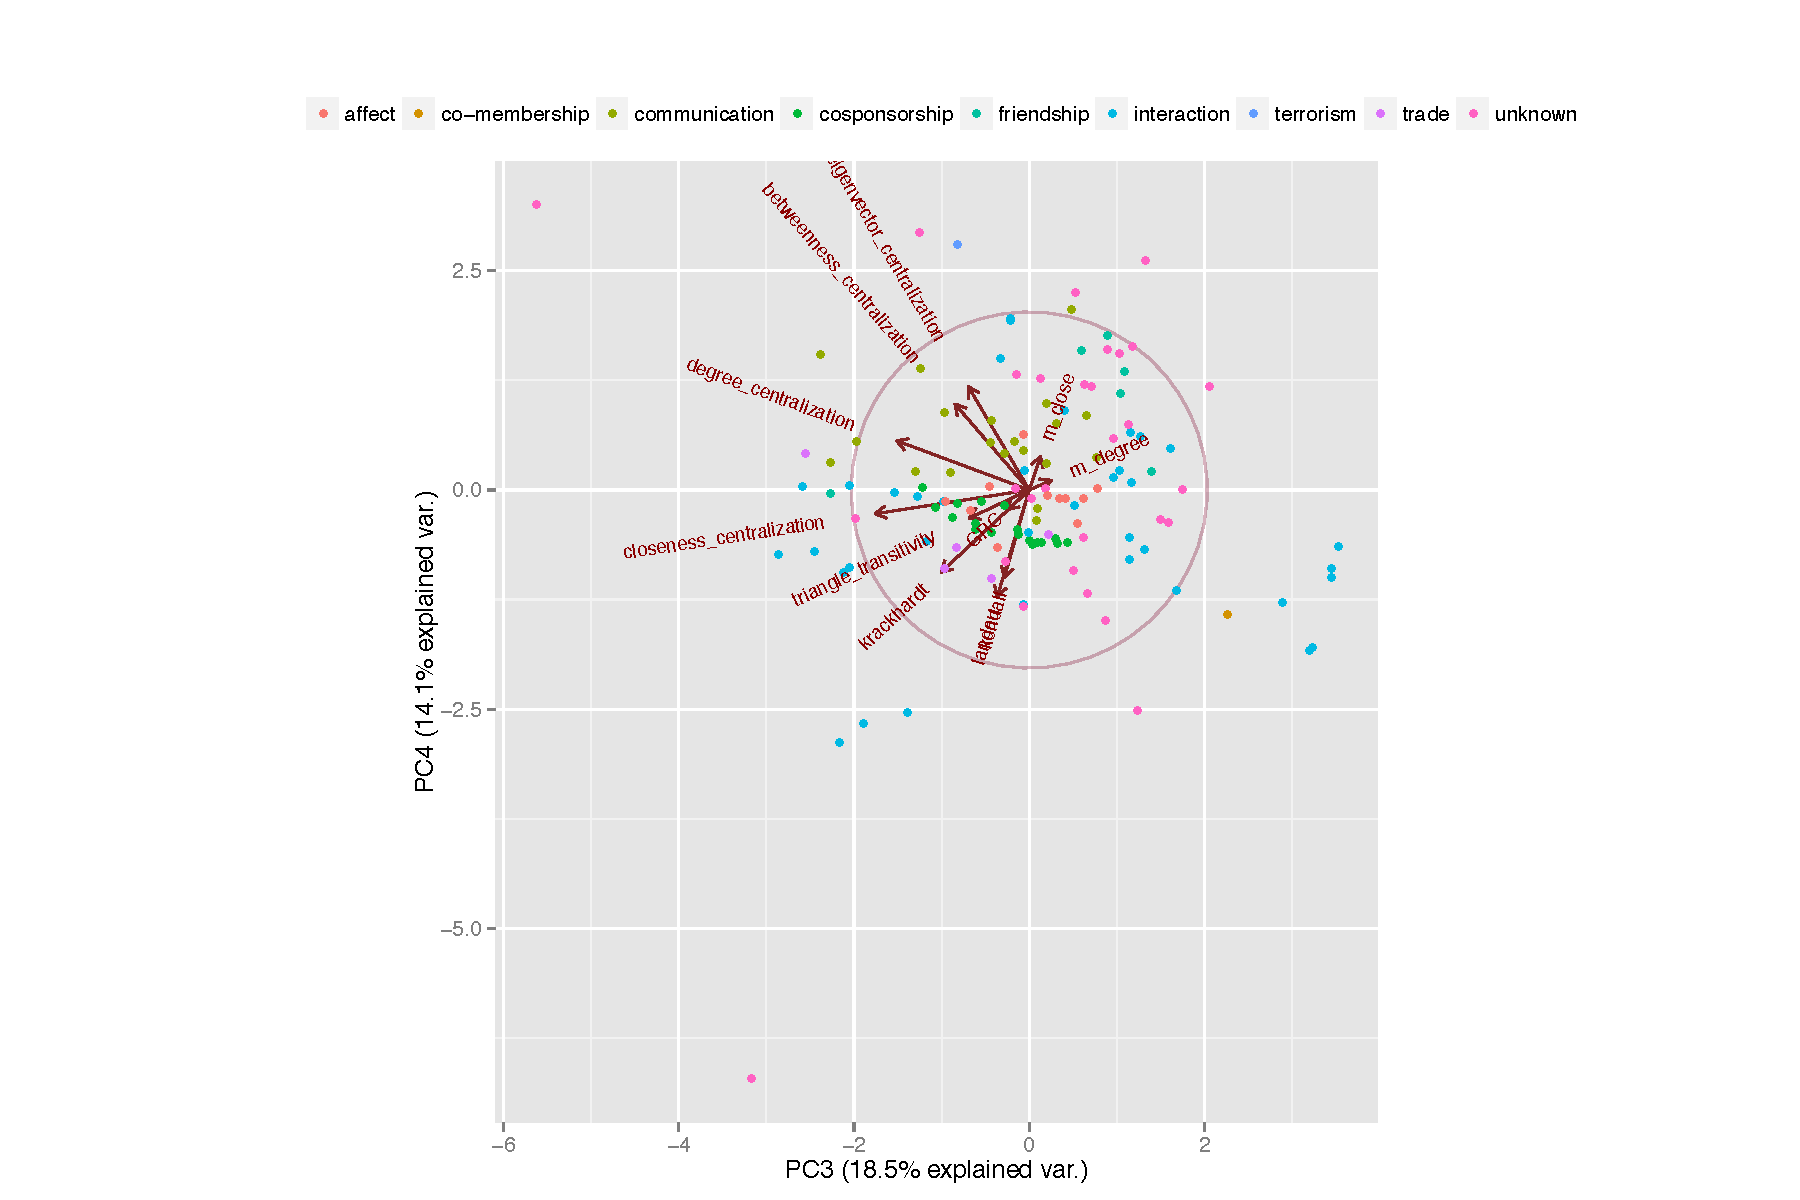
\includegraphics[width = 0.98\textwidth]{./images/Observed_PCA_Components3_4.pdf}
\end{center}
\end{figure}

\begin{figure}
\begin{center}
	\caption{\label{fig:rankings each county} Rankings scores for each county. The x-axis records how close to the top of the hierarchy a measure placed the county manager, with a higher score indicating better performance. Each column represents a different county.}
		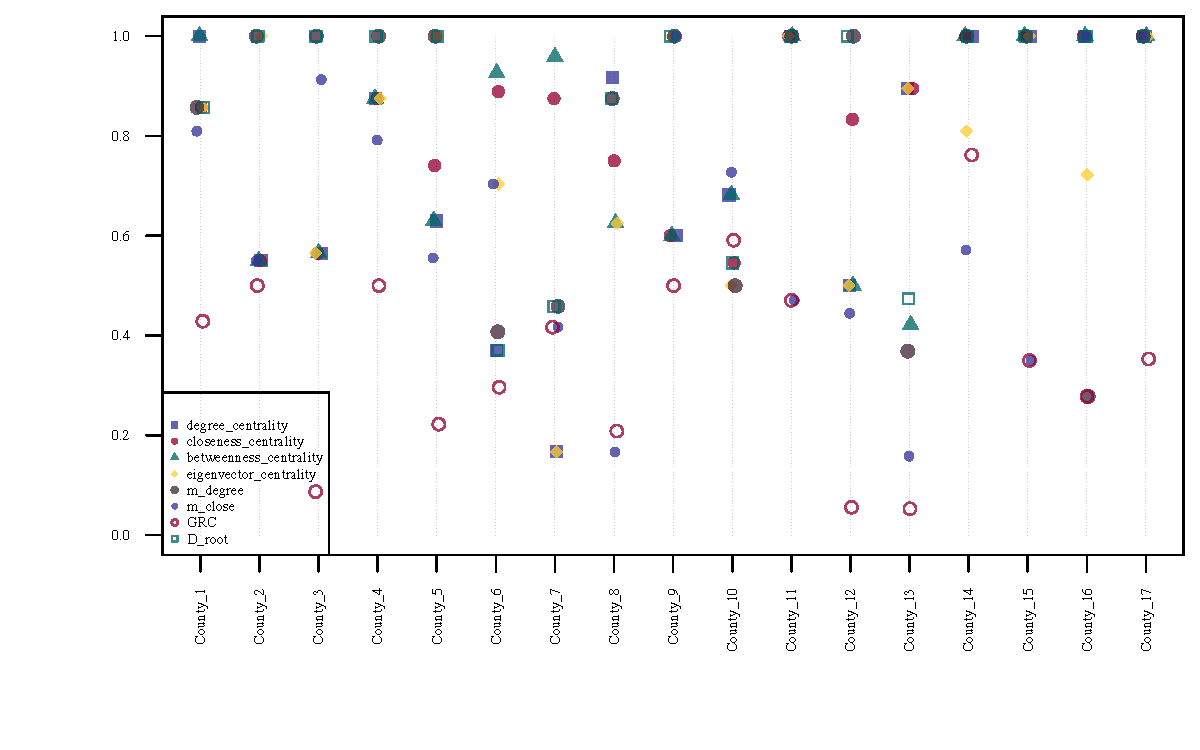
\includegraphics[width = 0.98\textwidth]{./images/Measure_Scores.pdf}
\end{center}
\end{figure}

% \section{Measure Pairs Plots}
% \label{sec:pairs plots}
%
% \begin{figure}[htp]
% \begin{center}
% 	\caption{\label{fig:pairs plots} Pairs plots between nine network hierarchy measures calculated on 136 networks. Points are colored according to network type, with the following color codings: \textbf{affect} = black,         \textbf{co-membership} = yellow,  \textbf{communication} = red, \textbf{bill cosponsorship} = orange, \textbf{friendship} = green,  \textbf{interaction} = blue, \textbf{terrorism} = pink, \textbf{trade} = maroon, and all networks for which the type was \textbf{unknown} were collored light brown.}
% 		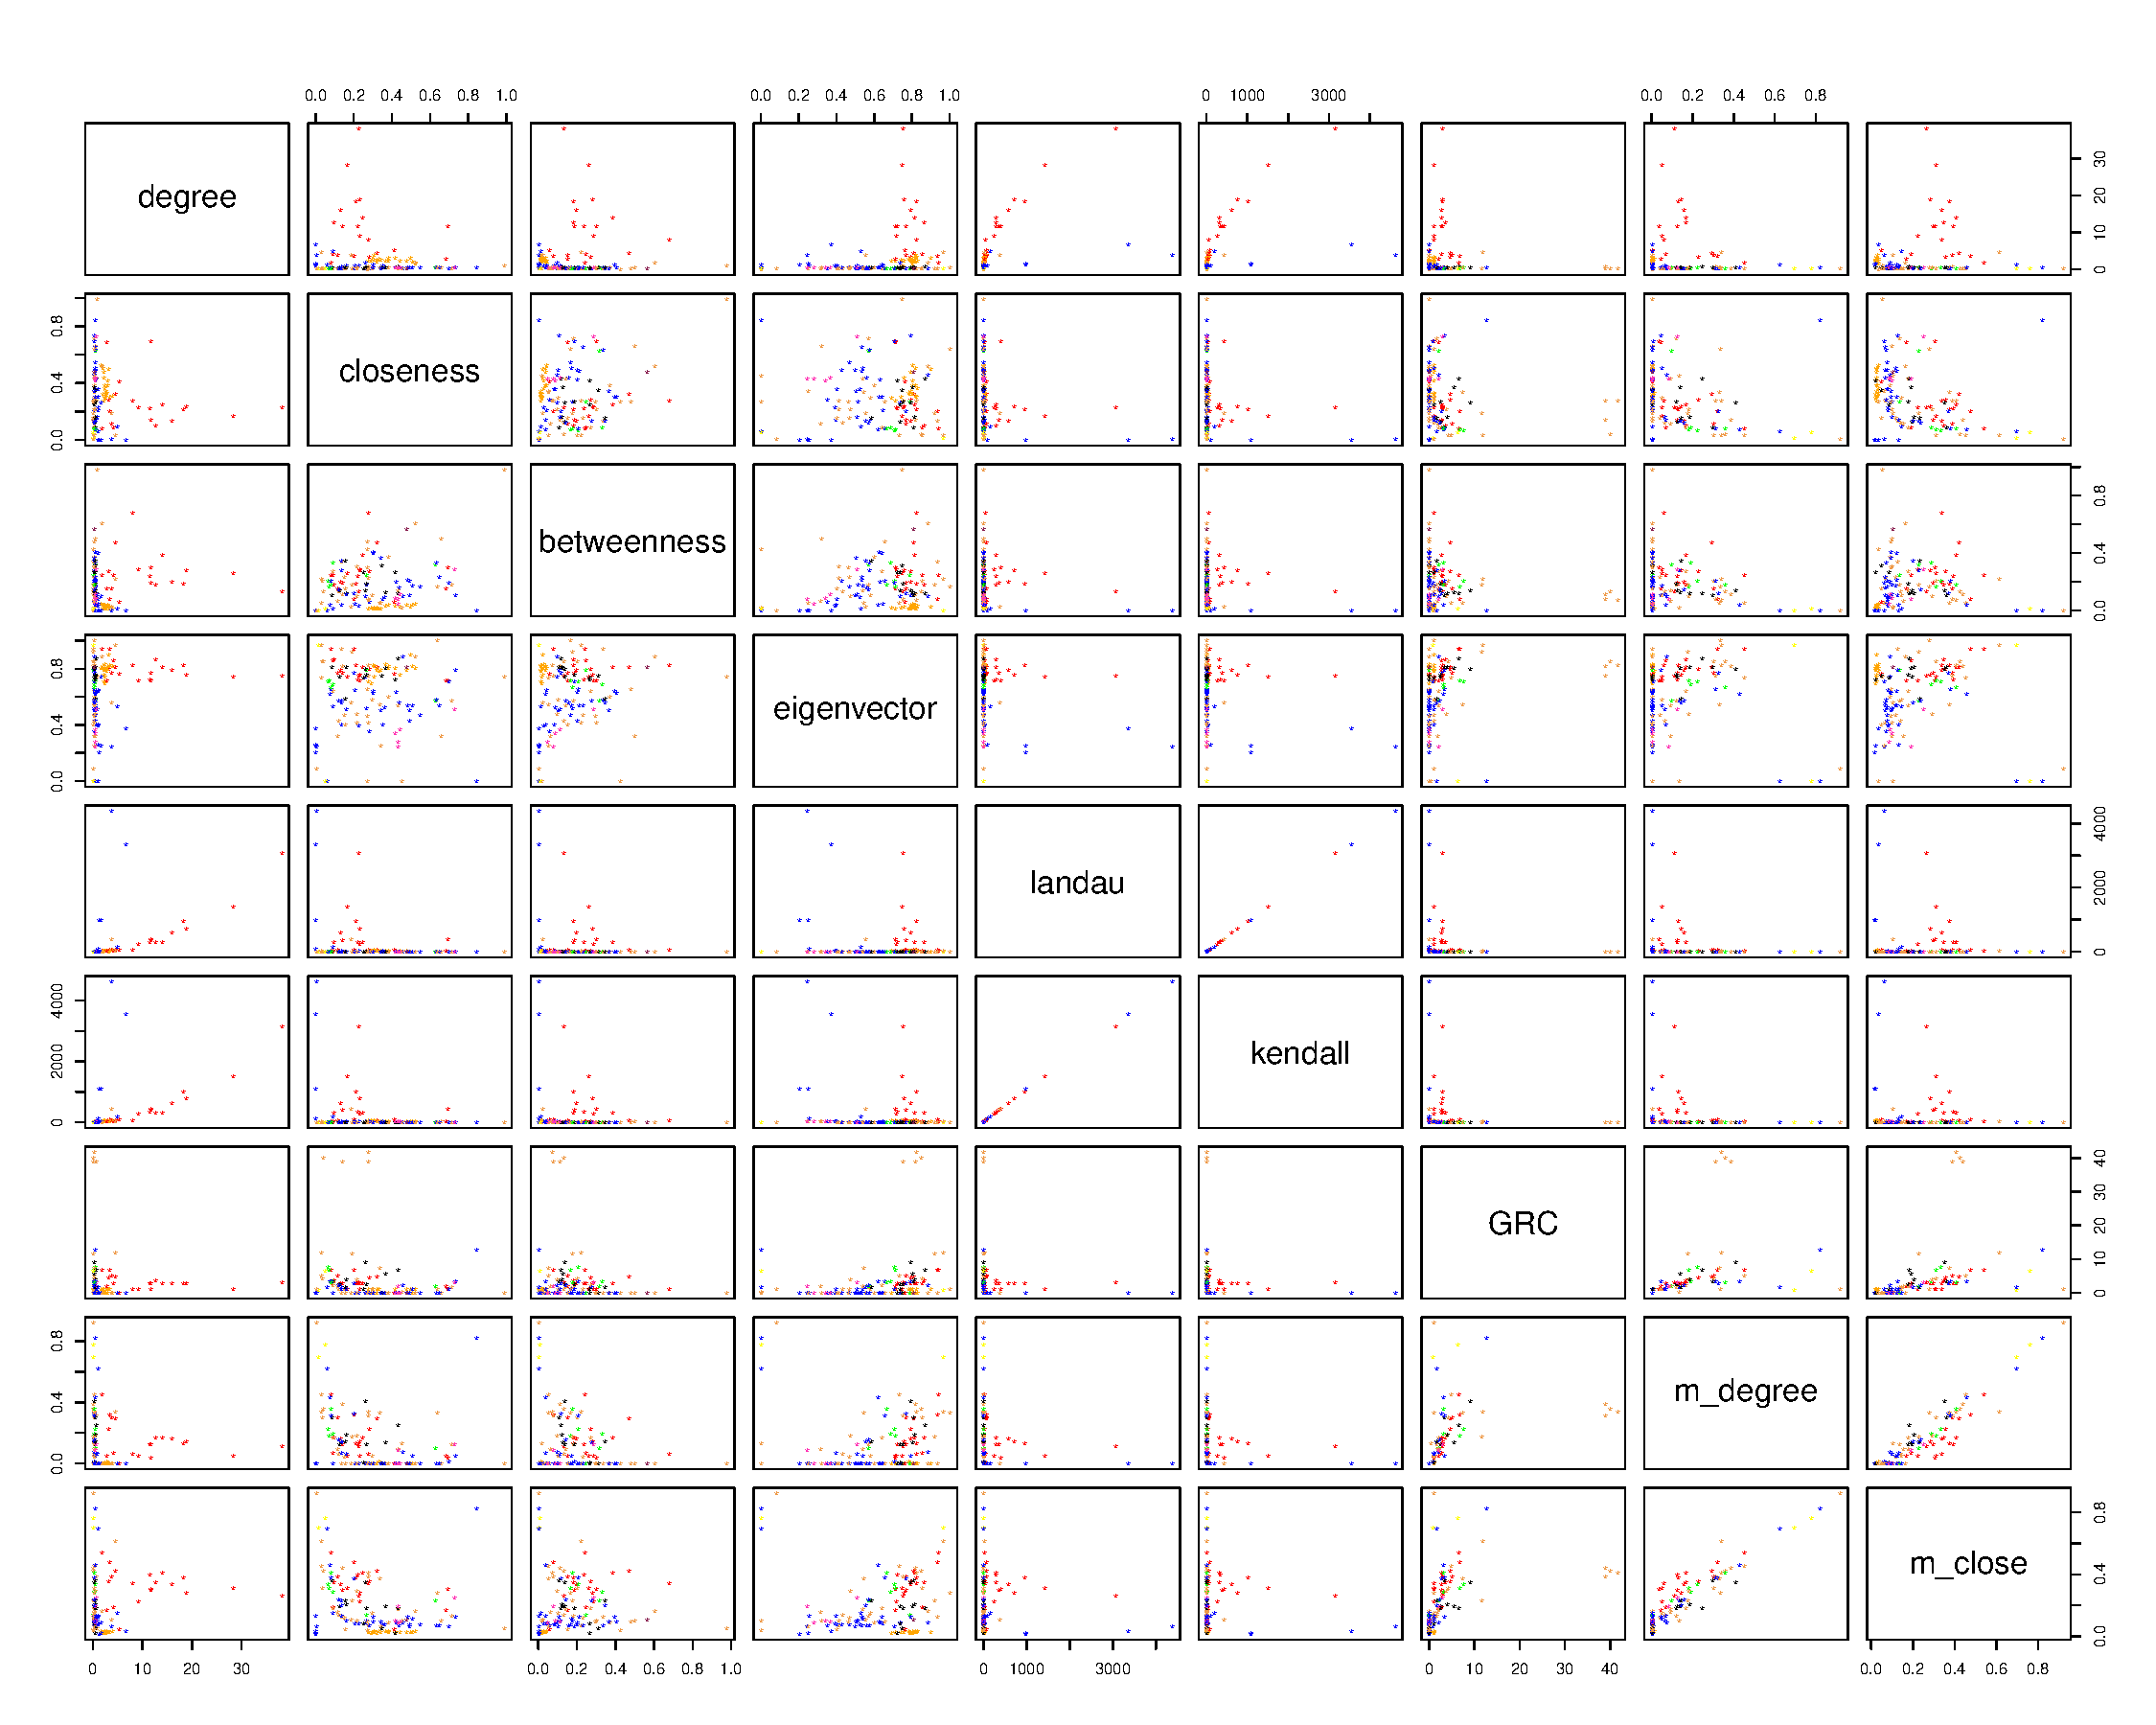
\includegraphics[width = 0.98\textwidth]{./images/Global_Measure_Pairs_Plots.pdf}
% \end{center}
% \end{figure}


% \section{Dataset References}
% \label{sec:dataset references}
%
% \begin{enumerate}
%
%
%
%     	\item Adolescent Health: survey asked students to list 5 male and female friends. \cite{AdHealth}
%
%     	\item Residence Hall: friendships between 217 students in Australian National University. \cite{Res}
%
%     	\item Taro Exchange: gift--giving relationships between households in a Papaun village. \cite{Taro}
%
%     	\item Highschool: friendship relationship between boys at a small Indiana high school in 1957-1958. \cite{HS}
%
%     	\item Dutch College: friendships between 32 university freshmen. \cite{Dutch}
%
%     	\item Monks: preference ratings between monks in a cloister during a crisis. \cite{monks}
%
%     	\item Physicians: innovation spread between 246 physicians in Illinois. \cite{docs}
%
%     	\item Seventh graders: activity specific proximity rankings for 29 middle school students in Victoria \cite{sevies}.
%
%     \item Prosper loans: loans between users of prosper.com \cite{prosper}.
%
%     \item Libimseti.cz: likes between users on a Czech dataing site \cite{libi}.
%
%     %\item Friendster: friendship adds on the online site Friendster \cite{friendster}.
%
%     \item Digg: friendships on Digg \cite{digg}.
%
%     \item Youtube: connections between Youtube users \cite{youtube}.
%
%     \item Epinions: who--trusts--whom between users of epinions \cite{epinions}.
%
%     \item EU emails: emails for 18 months from a major European research institution \cite{EU}.
%
%     \item Facebook: friends lists from FAcebook, generated through a Facebook app survey \cite{facebook}.
%
%     \item Google Plus: friends between users who selected to ``share circles'' on Google Plus \cite{facebook}.
%
%     \item Linx kernel mailing list: communication network for the linux kernel mailing list, where each edge is a reply from a user to another \cite{linux}.
%
%     \item Livejournal: map of an online community friendships of Livejournal users \cite{livejournal}.
%
%     \item Manufacturing: communication network between employess of a mid--size manufacturing firm \cite{manufacturing}.
%
%     \item Pokec: Friendship networks in the Pokec online social network, popular in Slovakia \cite{pokec}.
%
%     \item Slashdot: tagging between users in slashdot for 2008 and 2009 \cite{livejournal}.
%
%     \item Twitter: circles between twitter users \cite{facebook}.
%
%     \item UC Irvine: messages sent between students on an online community at UC Irvine \cite{irvine}.
%
%     \item U. Rovira i Virgili: email communication network from University Rovira i Virgili in Tarragona \cite{URV}.
%
%     %\item Wikipedia Talk: network of discussions between all users from the beginning of Wikipedia to January 2008 \cite{wiki}.
%
%     %\item Wikipedia Votes: data from administrator elections \cite{wiki}.
%
%     %\item Wikipedia Requests for Adminship: requests from 2003 through 2013 \cite{wiki2}.
%
%     %\item Friendster: network for online social site Friendster \cite{friendster}.
%
% \end{enumerate}



\end{document}

%%
%% End of file `ecrc-template.tex'. 
=======
When we understand societal processes and institutions under a theoretical framework oriented around social relations, we're actually invoking much of the main ideas of sociologist Michael Mann, who comprehends society as ``a network of social interaction" \cite{mann1986sources}. Mann's work in essence calls for a better discernment of the complexity of human social relations and needs, as opposed to Mann’s critique of past theories focusing too much as ``simple totalities" instead. Indeed, he says: ``Societies are constituted of multiple overlapping and intersecting sociospatial networks of power" \cite[p. 1]{mann1986sources}. In light of Mann's broader work, contemporary scholars note that ``[i]n terms of scope and ambition, this project [of Mann's] rivals the social thought of Marx and Weber" \cite[p. 338]{schroeder2007mann}, and his theorizing on the ``relations \textit{between} states" has filled a void that in general, ``[s]ociology has thus been unable to deal with [...] [regarding] contemporary social change" \cite[p. 339-340; emphasis>>>>>>> External Changes
